\pagestyle{empty}
\cleardoublepage
\pagestyle{fancy}

\selectlanguage{english}


\chapter{Genomic Perspective On Multivariate Variation, Pleiotropy, And Evolution}\label{capJoH}

Diogo Melo, Gabriel Marroig, Jason Wolf

\newpage

\vspace*{10pt}
% Abstract
\begin{center}
  \emph{\begin{large}Abstract\end{large}}
\vspace{2pt}
\end{center}

\noindent  
Multivariate quantitative genetics provides a powerful framework
for studying patterns and processes of phenotypic evolution. Quantitative
genetics parameters, like trait heritability or the G-matrix for sets of
traits, can be used to predict evolutionary response or to understand the
evolutionary history of a population. These population-level approaches have
proven to be largely successful, but the underlying genetics of multivariate
variation and evolutionary change typically remain a black box. Establishing a
deeper empirical understanding of how individual genetic effects lead to
genetic (co)variation is then crucial to our understanding of the evolutionary
process. To delve into this black box, we exploit an experimental population
of mice composed from lineages derived by artificial selection for body size.
We develop an approach to estimate the multivariate effect of loci and
characterize these vectors of effects in terms of their magnitude and
alignment with the direction of evolutionary divergence. Using these
estimates, we reconstruct the traits in the ancestral populations and quantify
how much of the divergence is due to the different kinds of genetic and
environmental effects. Finally, we also use these vectors to decompose
patterns of genetic covariation and examine the relationship between these
components and the corresponding distribution of pleiotropic effects. We find
that additive effects are much larger than dominance effects and are more
closely aligned with the direction of selection and divergence. Pleiotropic
effects are highly variable but are, on average, modular. These results are
consistent with pleiotropy being partly shaped by selection, while reflecting
underlying developmental constraints on patterns.

\par
\vspace{1em}
\noindent\textbf{Keywords:} G-matrix; QTL mapping; genome prediction; genetic architecture
\newpage

\begin{refsection}

\section{Introduction}

Individuals are composed of a complex array of traits that are interconnected
through shared genetic, physiological, and developmental processes.
Consequently, evolution is inherently a `multivariate' process, wherein suites
of traits interact to determine an individual's fitness. Differences in
fitness then generate selection that cascades to the genomic level through the
genotype-phenotype relationship, leading to heritable changes across
generations \parencite{Lande1983-ez,Klingenberg2008-ll,Melo2016-yw}.
Therefore, understanding evolutionary change in response to selection requires
deciphering the relationship between genotypic variation and multivariate
traits. The quantitative genetics framework was developed to achieve this
goal, historically relying on statistical measurement of genetic covariation
between traits as a summary of their genetic `connectedness'. The covariances
estimated using this framework can be used to describe how sets of traits
evolve together, including either for predicting the multivariate response to
selection \parencite{Lande1979-by}, or to retrospectively analyze divergence
by selective and neutral processes \parencite{Felsenstein1988-ql}. However,
this statistical framework treats the link between genotype and phenotype
underlying patterns of covariation as a `black box', and as a result, we still
have a relatively limited understanding of the underlying genetic architecture
of patterns of genetic covariation. Furthermore, patterns of genetic
covariation are themselves shaped by selection, which can lead to a complex
feedback between genetic architecture and evolution which we don't fully
understand \parencite{Turelli1994-pg,Jones2004-be,Jones2014-wj}. Therefore, an
explicit link between the properties of the individual loci that underlie the
multivariate genotype-phenotype relationship, and the associated consequences
for patterns of genetic covariation are central to the study of evolution.

To understand the patterns of genetic covariation between traits, studies have
historically taken a population level approach (top-down) that relies on
pedigree relations to dissect components of phenotypic covariation. These
studies are generally focused on how variation constrains evolution or how
variation itself evolves in relation to multivariate selection
\parencite{Arnold2008-pc,Futuyma2010-jl}. Whereas the effect of covariation in
constraining short term evolution is well established
\parencite{Lande1979-by,Grant1995-er,Schluter1996-gw} , we have only recently
begun to uncover the effects of covariation on macroevolution. Comparisons of
directions of divergence in several study systems have shown a remarkable
pattern of alignment between within population covariation and macro-
evolutionary divergence, with divergence being greater in directions of high
genetic variation, both in patterns of phenotypic
\parencite{Marroig2005-ce,Punzalan2016-lb,Simon2016-ed} and genetic
covariation \parencite{Houle2017-ph,McGlothlin2018-hm}. Whether this alignment
between divergence and covariation is a result of macroevolutionary
constraints limiting possible directions of evolutionary change, or due to
selection actively changing constraints using the available genetic variation
in patterns of covariation
\parencite{Arnold2001-lz,Pavlicev2011-xm,Pavlicev2015-up,Walter2018-dw}, or a
mixture of both, is still an open question. The extent to which genetic
covariation can evolve has been investigated in short term artificial (and
natural) selection experiments, that have shown that the G-matrix can quickly
evolve in response to selection
\parencite{Careau2015-sy,Assis2016-vz,Penna2017-if}, but there are also
examples of failure to increase multivariate variation via selection
\parencite{Sztepanacz2017-ot}. Given this rich scenario of experimental and
natural observations, a qualitative exploration of the sources and causes of
genetic covariation, and on how these constraints evolve, is fundamental to
furthering our understanding of diversification. Patterns of genetic
covariation between traits can be due to either pleiotropy (where a locus
affects more than one trait), or linkage disequilibrium (LD) (where alleles at
different loci affecting different traits tend to be co-inherited). Studies
generally assume the primacy of pleiotropy as a cause of long term genetic
covariation, because even relatively closely linked genes are expected to
reach linkage equilibrium over evolutionary timescales, and hence even when LD
is presence, its influence is likely to erode (unless actively maintained by
selection).

Although the potential causes of covariation are known, the population level
top-down approach only brings us indirect evidence of their contribution to
the structure and evolution of genetic covariation, and therefore we must then
rely on theoretical and computational models to infer how pleiotropy and LD
evolve under selection
\parencite{Barton1990-uu,Hansen2006-yc,Pavlicev2011-wz,Melo2015-bk}.
Quantitative trait locus (QTL) mapping and genome wide association studies
(GWAS) have begun to overcome this limitation, offering preliminary insights
into the genetic architecture underlying covariation (especially for growth
and morphological traits \parencite{Leamy2002-nh,Wolf2005-nr,Kenney-Hunt2008-bd,Porto2016-qc}. 
In these studies, the link between pleiotropy and
covariation has been made in a mostly qualitative manner using mapping
locations, with effects estimated using `univariate' models. Genomic regions
that are mapped on to more than one trait are considered pleiotropic, and the
observed covariation between these traits is related to this shared QTL. This
method, along with trait specific effect estimates for each QTL, has proven
very powerful for characterizing genetic architecture
\parencite{Wang2010-da,Wagner2011-kp}. For example, several studies have
pointed to a modular genotype-phenotype map, composed of predominantly local
genetic effects, as the main driver of variational modularity in growth and
morphological traits \parencite{Leamy2002-nh,Cheverud1996-fm,Mezey2000-rs}, in
opposition to the equally plausible hypothesis of compensatory antagonistic
and synergistic effects  that can lead to variational modularity via hidden
pleiotropy \parencite{Pavlicev2011-xm}, as was suggested in early quantitative
genetics analysis \parencite{Cheverud1983-fq}.

Advances in statistical and computational methods have started to change the
landscape of mapping approaches, with recent genome prediction and
regularization methods opting for using all available markers in large
prediction models, instead of mapping a small number of QTL of sufficiently
large effects \parencite{Meuwissen2001-cu,De_Los_Campos2013-gn}. In general,
genome prediction methods perform well in predicting phenotypes, but at the
cost of interpretability. Unlike mapping models, genome prediction distributes
the genetic effects across all markers and does not identify specific QTL
linked markers (this could be done after the model fitting by some variable
selection procedure like in \textcite{Piironen2015-ai} or
\textcite{Moser2015-sm}  but doing so is uncommon). GWAS and QTL mapping
methods have also advanced, with several mixed-model association methods
allowing for the efficient analysis of a very large number of markers in
structured populations \parencite{Lipka2012-tf,Zhou2012-zl,Lippert2011-jn} ,
all with good statistical performance \parencite{Eu-Ahsunthornwattana2014-fn}.
However, these genome prediction and mixed-model association methods still
deal poorly with multiple traits, and so we are limited to the traditional
method of mapping traits separately and assessing pleiotropy \emph{post-hoc}.
These shortcomings may be overcome in the near future, with some promising
methods being developed for efficient multivariate mapping
\parencite{Pitchers2017-ge,Hannah2018-zh,Kemper2018-gi}. Multivariate mapping
is fundamental for a qualitative study of pleiotropy, as it allows for
detection of QTL with large effects overall but small effects on each
individual trait under investigation. Multivariate mapping, when combined with
quantitative genetics theory, also allows for a direct quantification of the
effects of pleiotropic genetic effects on covariation, providing a much finer
description of the genetic basis  of covariation when compared to simple
mapping of common QTL.

Here, we develop a multivariate mixed model framework to understand the
genetic basis to patterns of covariation among growth traits in a mouse cross.
Growth and size have long been ideal models for the study of genetic
architecture, for several reasons. First, size is very amenable to artificial
selection, having standing heritable variation and being easy to measure by
several proxies, such as weight or length. Second, organismal growth unfolds
through various stages, and these stages have different mechanisms and
timings. For example, early quantitative genetics selection experiments showed
that changes in cell number and cell size were somewhat independent mechanisms
for changing the final size of the population under selection
\parencite{Falconer1978-kq,Cheverud1983-fq,Leamy1984-df,Riska1984-ml}. These
stages of development can then be considered as several related traits
interacting to form the final phenotype. Third, the  covariation that exists
between the different stages of growth (like early and late growth) provides
an ideal system to investigate the relation between pleiotropy and
covariation. We primarily focus on a QTL mapping model to study the
distribution of pleiotropic effects in order to link the pleiotropic effects
of individual loci to the covariation between traits and to evolutionary
change. We also adapt our mapping approach to fit a genome prediction model,
allowing us to examine the differences and advantages of these alternative
approaches. We apply these models to a population of mice derived from an
intercross of mouse strains that diverged in size by univariate directional
selection. By focusing on traits related to population divergence, we are able
to place our genetic analyses in an evolutionary context. By using this
explicit bottom-up approach to relate pleiotropy, selection and covariation,
we ask: how malleable are patterns of covariation between traits? How much do
they change under selection? Do patterns of pleiotropy align with selection or
do they reflect developmental constraints? Can we use segregating variation to
reconstruct the ancestral states of populations diverging by selection? All
these questions help us come to a richer understanding of variation and of the
evolutionary processes.


\section{Methods}

\subsection{Study population}

Our focal population is comprised of 1548 animals from the
F\textsubscript{3} generations of an intercross between the inbred LG/J
and SM/J strains if mice (for details see \textcite{Cheverud1996-fm,Wolf2008-cq}.
These strains were derived independently by
artificial selection for large (LG/J strain derived by \textcite{Goodale1938-an} or small
(SM/J strain derived by \textcite{MacArthur1944-ew} body weight
at 60 days of age (see  \textcite{Chai1956-fy}).
They differ by ca. 8.5 within-strain standard deviations in
adult body weight (at 63 days of age) \parencite{Kramer1998-cc}. For
simplicity, we refer to the lines as Large (LG/J) and Small (SM/J).

Details of the genotyping are provided by Wolf et al. (2008) and are
only briefly outlined here. Each individual was genotyped at 353 SNP
loci distributed across the 19 autosomes. Genotypes at each locus
(\emph{LL}, \emph{LS} and \emph{SS}, with the `\emph{L}' allele coming
from Large and the `\emph{S}' allele coming from Small) were assigned
additive (\emph{X\textsubscript{a}}) and dominance
(\emph{X\textsubscript{d}}) genotypic index values, where the values of
\emph{X\textsubscript{a}} are \emph{LL} = +1, \emph{LS} and \emph{SL} =
0, \emph{SS} = --1, and for \emph{X\textsubscript{d}} are \emph{LS} and
\emph{SL} = 1, \emph{LL} and \emph{SS} = 0 (see Wolf et al. 2008)

Animals were weighed weekly from one week of age. Our analyses focus on
weight gained over each one week interval (`growth') from one week to
seven weeks of age. These growth traits were calculated simply as the
absolute difference in body weight between the weeks that define each
time interval (e.g., growth\textsubscript{1,2} = weight\textsubscript{2}
- weight\textsubscript{1}). See \textcite{Vaughn1999-wt} and \textcite{Hager2009-mz}
 for further details.

\subsection{Phenotypic divergence}

The vector of phenotypic divergence between founders was estimated as
the difference between the means of the phenotypes of the founders. To
estimate the direction of selection, we used a multiple regression of
the growth traits in the F\textsubscript{3} with the target of
selection, week 9 weight, and used the partial regression coefficients
as the expected direction of the selection gradient \parencite{Lande1983-ez}. By multiplying this
selection gradient to the observed G-matrix we also obtained an expected
phenotypic divergence, which can be compared to the observed divergence.
We also scaled the selection gradient so that the norm of the expected
divergence vector is the same as the observed vector. This scaling is
necessary because the magnitude of selection estimated by the multiple
regression is too small to account for the many generations of
selection. Using these multivariate vectors of selection and divergence,
we measured the alignment of the estimated genetic effects (see below), phenotypic
divergence and selection gradients. This allows us to characterize the 
genetic basis of the phenotypic divergence due to selection. Alignment between vectors was measured
using vector correlations, that is, the cosine of the angle between the
vectors being compared. We also investigate the relation between the
norm of the pleiotropic effect vector and its alignment with the
directions of selection and divergence.

\subsection{Loci and alleles}

We build our analysis on the classic quantitative genetic framework
using a model of \emph{n} biallelic loci that affect the value of
\emph{t} traits. At each \emph{j}th locus we label alleles
as \(L_{j}\) and \(S_{j}\) to indicate the allele originating from the Large
and Small strains respectively. The frequencies of alleles are given
by \(p_{j}\) for \(L_{j}\) and \(q_{j}\) for \(S_{j}\). To build a multi-locus
model we assemble genotypes from the four possible haplotypes at each
pair of loci: \(H_{L_{j}L_{x}}\), \(H_{L_{j}S_{x}}\), \(H_{S_{j}L_{x}}\), and \(H_{S_{j}S_{x}}\) (hence
the multi-locus genotype is assembled from pairwise combinations of
loci). The frequencies of the four haplotypes at each locus pair depends
on the frequencies of alleles at the two loci and the extent of linkage
disequilibrium, such
that: \(H_{L_{j}L_{x}} = p_{j}p_{x} + \lambda_{jx}\), \(H_{L_{j}S_{x}} = p_{j}q_{x} - \lambda_{jx}\), \(H_{S_{j}L_{x}} = q_{j}p_{x} - \lambda_{jx}\), and \(H_{S_{j}S_{x}} = q_{j}q_{x} + \lambda_{jx}\), where \(\lambda_{jx}\) is a measure of LD defined as: \(\lambda_{jx} = H_{L_{j}L_{x}}H_{S_{j}S_{x}} - H_{L_{j}S_{x}}H_{S_{j}L_{x}}\).

\subsection{Genetic effects}

Genotypes at each locus, \emph{j}, (listed as
\(L_{j}L_{j},L_{j}S_{j},S_{j}S_{j}\)) were assigned additive
(\(X_{j}^{a} \in \lbrack 1,\ \ 0,\ \  - 1\rbrack\)) and dominance
(\(X_{j}^{d} \in \lbrack 0,\ \ 1\rbrack\)) index values, such that:

\begin{equation}
\begin{bmatrix}
\overline{L_{j}L_{j}} \\
\overline{L_{j}S_{j}} \\
\overline{S_{j}S_{j}} \\
\end{bmatrix} = \begin{bmatrix}
1 & 1 & 0 \\
1 & 0 & 1 \\
1 & - 1 & 0 \\
\end{bmatrix}\begin{bmatrix}
r_{j} \\
a_{j} \\
d_{j} \\
\end{bmatrix}
\end{equation}

where the overbar indicates the average phenotype associated with each
genotype (i.e., the `genotypic value' for each), which yields estimates
of the additive and dominance genetic effects corresponding to the
standard definition \parencite{Falconer1996-ot}

\begin{equation}
\begin{bmatrix}
r_{j} \\
a_{j} \\
d_{j} \\
\end{bmatrix} = \begin{bmatrix}
\frac{\left( \overline{L_{j}L_{j}} + \overline{S_{j}S_{j}} \right)}{2} \\
\frac{\left( \overline{L_{j}L_{j}} - \overline{S_{j}S_{j}} \right)}{2} \\
\overline{L_{j}S_{j}} - \frac{\left( \overline{L_{j}L_{j}} + \overline{S_{j}S_{j}} \right)}{2} \\
\end{bmatrix}
\end{equation}

The additive and dominance effects (i.e., genotypic values, defined in
equation 2 above) of locus \emph{j} were estimated as effects from a
linear model:

\begin{equation}
E\left\lbrack z_{i} \right\rbrack = r_{j} + a_{j}X_{ij}^{a} + d_{j}X_{ij}^{d} + \varepsilon_{ij}
\end{equation}

where \(z_{i}\) indicates the
phenotypic value of individual \emph{i},\(\ r_{j}\) the reference point
(representing the intercept), \(\ X_{ij}^{a}\) the additive and
\(X_{ij}^{d}\) the dominance genotypic index values for
individual \emph{i} at locus \emph{j}, and \(\varepsilon_{ij}\)
the residual. Equation (3) can be extended to a multivariate form:

\begin{equation}
E\left\lbrack \textbf{Z}_{i} \right\rbrack = \textbf{r}_{j} + \textbf{a}_{j}X_{ij}^{a} + \textbf{d}_{j}X_{ij}^{d} + \pmb \varepsilon_{ij}
\end{equation}

Where \(Z_{i}\) is the vector (with length \emph{t}) of traits measured
for individual \emph{i}. This model provides estimates of the vectors of
additive
(\(\textbf{a}_{j} = \left\lbrack a_{1(j)}\ \ldots\ a_{t(j)}\  \right\rbrack\))
and dominance
(\(\textbf{d}_{j} = \left\lbrack d_{1(j)}\ \ldots\ d_{t(j)}\  \right\rbrack\))
effects, which summarize the pleiotropic effects of locus \emph{j}
across the \emph{t} traits.

\subsection{QTL mapping}

We identified candidate QTL for the growth traits by fitting
multivariate linear mixed models using dam as a random effect, and using
separate fixed terms for the additive and dominance effects of the loci
under consideration, as in equation (3) and (4). The simple family-level
random effect controls for relatedness because all families in the
F\textsubscript{3} are equally related. To estimate the QTL location, we
used interval mapping models, by including flanking markers at various
distances on either side of the focal marker (5, 10, 15 and 20 cM).
Significance was assessed by dropping the focal marker and using a
likelihood ratio test (LRT) with a Satterwhite correction. Models were
fit in the R programming language using the lme4 package \parencite{Bates2008-gp}, and
the LRT was performed in the lmerTest package \parencite{Kuznetsova2017-fq}. We
calculate chromosome-wise and genome-wise significance using a
Bonferroni correction with the effective number of markers in each
chromosome and in the whole genome. This method takes the correlation
between markers (LD) into account when setting the overall significance
threshold \parencite{Nyholt2004-zm,Li2005-yu}. A list of markers and code for performing the mapping
is available in the supporting information (SI).

Using the list of candidate markers, we then estimated the effects of each
marker in all of the traits using a Bayesian multiple multivariate regression,
again with family as a random effect. We used unit normal priors on the
regression coefficients, centered Cauchy priors with unit scale on the
variances and LKJ priors with scale 4 on the genetic and residual correlations
between traits. This produces two vectors of effects for each marker on each
trait, one for additive effects and one for dominance effects. We call these
effect vectors pleiotropic vectors, as they measure the full pleiotropic
effects of all the significant markers on the observed traits. This multiple
regression was done in Stan \parencite{Carpenter2017-pn} using custom code,
also available in the SI\footnote{Code for fitting the models is available in
\url{https://github.com/diogro/mouseGrowthQTLs}.}.

\subsection{Genome prediction}

For the genome prediction, instead of running single marker models to select
candidate markers, we ran one full model with all of the markers and used
hierarchical shrinkage priors to produce regularized per-marker coefficients.
Regularized coefficients are either heavily shrunken towards zero, indicating
that the marker has no effect on a particular trait, or not shrunken,
estimating the putative effect of that marker on a trait. This produces
pleiotropic vectors for each marker in our model, but most of the coefficients
in these pleiotropic vectors were close to zero. We implemented a custom
version of the regularized horseshoe prior in Stan using the recommendations
in \textcite{Piironen2017-ih}. This allowed us to include the family level
random effect that accounts for relatedness and to partition the marker effect
into an additive and a dominance components.

\subsection{Estimation of quantitative genetic parameters}

The genetic variance-covariance matrix was estimated from the null QTL
mapping model (see above), where the same model was fitted without any
marker information included. This provides a family-level estimate of
the genetic covariance matrix based on the covariance of full siblings. Because it is
based on full siblings, it does not provide a direct estimate of the
additive genetic variance-covariance matrix (i.e., the G-matrix).
Rather, it is composed of one half of the additive genetic covariance
matrix plus one quarter of the dominance genetic covariance matrix, plus
any covariation due to shared environment within families. Therefore, we
refer to this as the `full-sib' genetic variance-covariance matrix.

\subsection{Ancestral trait reconstruction}

As a test of the quality of the pleiotropic genetic effect we estimated
in the QTL mapping and genome prediction model, we used the estimated
pleiotropic vectors to predict the phenotype in the ancestral founder
populations of the Large and Small mice. We can predict the phenotype of
the ancestral lines by asking what the phenotype of an individual of the
F\textsubscript{3} generation would be if this individual had only Small
or Large alleles. Both the QTL mapping and genome prediction models
provide estimates of vector of additive effects of all loci on all
traits. Each additive effect corresponds to half the difference between
the average phenotypes of the alternative homozygotes. Therefore, the
vector of additive effects can be multiplied by the index value of {+1} to
yield the estimated trait value of a Large allele homozygote across all
loci, as a deviation from the F\textsubscript{3} mean (which represents
the average reference point for the model). Likewise, multiplying the
vector of additive effects by an index value of {-1} yields an estimate of
the phenotypic value of the Small allele homozygote across all loci
(again, as a deviation from the mean).

\begin{equation}
E\left\lbrack Z_{LL} \right\rbrack = \mu + \sum_{j=1}^n a_{j}
\end{equation}

and

\begin{equation}
E\left\lbrack Z_{SS} \right\rbrack = \mu + \sum_{j=1}^n -a_{j}
\end{equation}

\subsection{Estimation of genetic (co)variances}

To separate heritable (additive) from non-heritable (dominance) genetic
variation we first define the average effect of an allele substitution
(\(\alpha_{j}\)), which corresponds to the expected change in the value
of each of the \emph{t} traits resulting from replacing an \emph{S}
allele with an \emph{L} allele. The vector \(\alpha_{j}\) therefore
summarizes the heritable (pleiotropic) effect of a locus since it
reflects how changing an allele at a locus would, on average, change the
phenotype of an individual. Although the genetic effects (\(a_{j}\) and
\(d_{j}\)) are a property of the locus, the average effect of an allele
substitution depends on the frequencies of alleles in a population:

\begin{equation}
\alpha_{j} = \textbf{a}_{j} + \left\lbrack q_{j} - p_{j} \right\rbrack \circ \textbf{d}_{j}
\end{equation}

Where \(\circ\) indicates the Hadamard (element wise) product, which
yields

\begin{equation}
\mathbf{\alpha}_{j}\mathbf{=}\begin{bmatrix}
a_{1(j)} + d_{1(j)}(q_{j}{- p}_{j}) \\
 \vdots \\
a_{t(j)} + d_{t(j)}(q_{j}{- p}_{j}) \\
\end{bmatrix}
\end{equation}

Equations (7) and (8) emphasize that the additive genetic variance
contains two components, one caused by the additive effects and one
caused by dominance effects.

Each $j$th locus contributes to the additive,
\(G_{k} = 2p_{j}q_{j}\alpha_{k(j)}^{2}\), and
dominance, \(D_{k} = \left( 2p_{j}q_{j}d_{k(j)} \right)^{2}\), genetic
variances of trait \emph{k.} Likewise, each locus contributes to the
additive, \(G_{kl} = 2p_{j}q_{j}\alpha_{j(k)}\alpha_{j(l)}\) ,
and dominance,
\(D_{kl} = \left( 2p_{j}q_{j}d_{k(j)}d_{l(j)} \right)^{2}\),
genetic covariances between traits \emph{k} and \emph{l}. The individual
contributions of loci can be summed to yield the total additive and
genetic (co)variances if loci are independent. However, when there is
linkage disequilibrium there will be an additional component of
(co)variation:

\begin{equation}
G_{kk} = \sum_{j=1}^n 2p_{j}q_{j}\alpha_{j(k)}^{2} + \sum_{j=1}^n \sum_{x=1}^n \left\lbrack {2\lambda_{jx}\alpha}_{j(k)}\alpha_{x(k)} \right\rbrack_{j \neq x}
\end{equation}

The second term on the RHS is summed over all pairs of loci not
including a locus with itself (hence the condition given that
\(j \neq x\)), given that \(\lambda_{jx} = \lambda_{xj}\).
The first summation term on the RHS of equation (9) represents the
contribution of individual loci to the total additive genetic variance,
while the second term represents the additional variation caused by LD
between loci. This latter term essentially represents the allelic
covariance between loci, such that the total additive genetic variance
is composed of a term arising from the effect of allelic variation
(hence it being weighed by the squared average effect) and a term
arising from the allelic covariance among loci (weighted by the product
of the average effects of the alleles).

As for the off diagonal terms, the additive genetic covariance between
traits \emph{k} and \emph{l} is given by:

\begin{equation}
G_{kl} = \sum_{j=1}^n 2p_{j}q_{j}\alpha_{j(k)}\alpha_{j(l)} + \sum_{j=1}^n \sum_{x=1}^n \left\lbrack {2\lambda_{jx}\alpha}_{j(k)}\alpha_{x(l)} \right\rbrack_{j \neq x}
\end{equation}

The dominance genetic variance, like the additive genetic variance,
contains a component arising from allelic variation and a component
caused by linkage disequilibrium:

\begin{equation}
D_{kk} = \sum_{j=1}^n \left( 2p_{j}q_{j}d_{j(k)} \right)^{2} + \sum_{j=1}^n \sum_{x=1}^n \left\lbrack 4\lambda_{jx}^{2}d_{j(k)}d_{x(k)} \right\rbrack_{j \neq x}
\end{equation}

Like for the dominance genetic covariance:

\begin{equation}
D_{kl} = \sum_{j = 1}^{t}{\left( 2p_{j}q_{j} \right)^{2}d_{j(k)}d_{j(l)} + \sum_{j = 1}^{n}{\sum_{x = 1}^{n}{\left\lbrack 4\lambda_{jx}^{2}d_{j(k)}d_{x(l)} \right\rbrack_{j \neq x}}}}
\end{equation}


From these definitions for the additive genetic variances and
covariances, we can construct the additive genetic variance covariance
matrix:

\begin{equation}
\mathbf{G} = \begin{bmatrix}
G_{11} & \cdots & G_{1t} \\
 \vdots & \ddots & \vdots \\
G_{t1} & \cdots & G_{tt} \\
\end{bmatrix}
\end{equation}

And the dominance genetic variance-covariance matrix:

\begin{equation}
\mathbf{D} = \begin{bmatrix}
D_{11} & \cdots & D_{1t} \\
 \vdots & \ddots & \vdots \\
D_{t1} & \cdots & D_{tt} \\
\end{bmatrix}
\end{equation}

Because the full-sib genetic variance-covariance matrix estimated using
the mixed model in the F\textsubscript{3} population represents a
mixture of additive and dominance components (see above), it is
estimated as the sum ½ \textbf{G} + ¼ \textbf{D} from equations (13)
and (14). Because the G matrix itself contains components arising from
additive and dominance effects, we also calculated the additive genetic
variance due to additive effects, \(G^{a}\), and dominance effects,
\(G^{d}\) by setting the additive (\(a_{j}\)) or dominance (\(d_{j}\))
effects to zero.

\subsection{Matrix comparisons}

To evaluate the quality of the matrix estimates, we compare the estimated covariance matrices using three complementary
methods, which focus on different aspects of matrix structure. The
Random Skewers method \parencite{Cheverud2007-yp} summarizes the extent to which matrices are
similar in the direction of their expected response to selection. This is done by
multiplying the two matrices being compared by the same set of random
selection gradients and taking the average of the vector correlations
between the resulting expected response vectors. Significance of the
Random Skewers comparison is calculated by comparing the observed vector
correlation to the distribution of correlations from random vectors. The
next method is a simple element wise correlation of matrix elements,
which can be used in correlation matrices as a measure of the similarity
in the pattern of association. Significance of the matrix correlation is
done using the Mantel permutation method, with takes the
non-independence of the individual elements in the matrix into account.
The Krzanowski correlation measures the congruence of the spaces spanned
by the first half of the eigenvectors of the matrices being compared. We
do not calculate a significance in relation to the Krzanowski method.
See \parencite{Melo2015-kf} for details on all these comparison methods.

\section{Results}

\subsection{Growth curves}

Growth curves for the parental and F\textsubscript{3} generation suggest
an almost completely additive behavior of the weekly growths, with the
F\textsubscript{3} generation being intermediate between the two
founders for most traits, except for the first week, in which the
F\textsubscript{3} generation is smaller than both founders (Fig.~\ref{fig:joh:growth}A).
Genetic correlations between growth periods are generally positive,
except for a negative correlation of -0.36 between growth in weeks 2 and
4. Larger correlations are present in later growth (around 0.3 to 0.4 in
adjacent weeks and between weeks 4 and 6). Early growth shows a positive
correlation between weeks 2 and 3. Most correlations between early and
late growth are small, except for a .34 correlation between weeks 1 and
5. There is also a small negative correlation between weeks 2 and 6 (Fig.~\ref{fig:joh:growth}B).
In summary, during early growth week 1 is mostly
independent, weeks 2 and 3 are positively correlated; and during late
growth and weeks 4-7 are positively correlated and somewhat independent
of early growth.

\begin{figure}
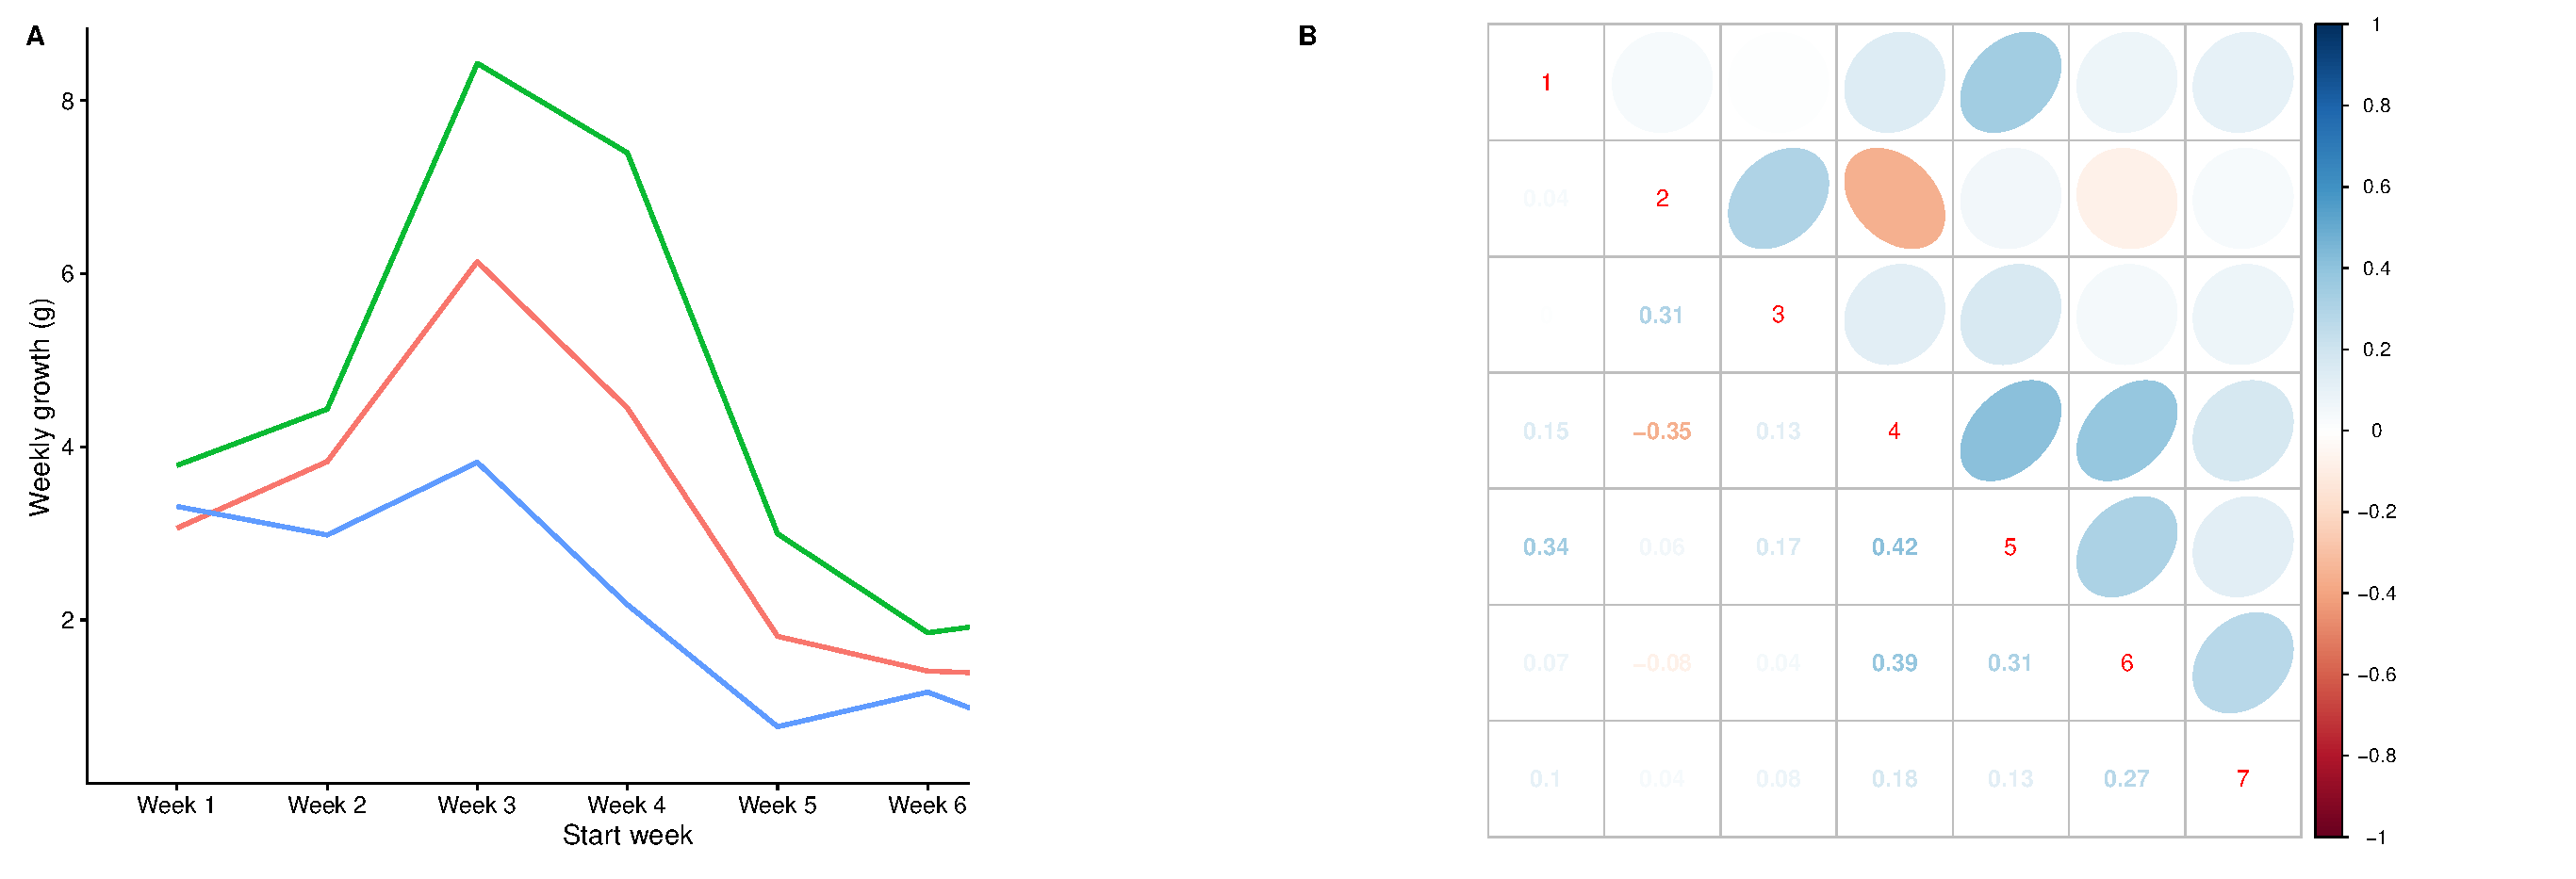
\includegraphics[width=\linewidth]{chapter_JoH-Melo_etal/media/growth_LG_SM_F3_covF3.eps}
\caption[Growth curves]{Growth curves. (A) Weekly growth for the founders (Large
shown in the top line (green), and Small in the lower line (blue)) and the
F\textsubscript{3} generations (middle line, red). In most growth periods,
the F\textsubscript{3} generation is between the two founders. (B)
Genetic correlations from the full-sib genetic matrix in the
F\textsubscript{3} generation. Smaller correlations are more transparent
and related ellipses less eccentric, larger correlations are more opaque
and ellipses more eccentric. Positive correlations in blue and negative
correlations in red.}
\label{fig:joh:growth}
\end{figure}

\subsection{Selection and divergence}

The observed phenotypic divergence, the estimated selection gradient and
the expected phenotypic divergence given this gradient are shown in
Table~\ref{joh:vectors} and Fig.~\ref{fig:joh:divergence}. Vector correlation between observed and expected
phenotypic divergence is high (\emph{r} = 0.93), indicating that the observed
divergence is compatible with the expected from selection and
covariation in the F\textsubscript{3}.

\begin{table}[htbp]
	\caption[Evolutionary vectors]{Vectors of phenotypic divergence, estimated selection gradient
			 in the F\textsubscript{3} and expected divergence given the estimated
			 selection.}
	\vspace{1em}
	\centering
	\begin{tabular}{l|p{30mm} p{30mm} p{40mm}}
		\toprule
		Week interval & Observed \newline divergence (g) $\Delta z$ & Estimated \newline selection gradient (scaled) & Expected \newline phenotypic divergence \\
		\midrule
		Week 1 - 2 & 0.475 & 3.336 & 1.221 \\
		Week 2 - 3 & 1.455 & 7.377 & 2.823 \\
		Week 3 - 4 & 4.610 & 7.666 & 3.986 \\
		Week 4 - 5 & 5.220 & 6.146 & 3.947 \\
		Week 5 - 6 & 2.230 & 6.606 & 3.178 \\
		Week 6 - 7 & 0.685 & 5.982 & 2.348 \\
		Week 7 - 8 & 1.575 & 4.323 & 1.494 \\
		\bottomrule
	\end{tabular}
	\label{joh:vectors}
\end{table}

\subsection{QTL mapping}

We identified 32 putative QTL loci using our multivariate regression
model with flanking markers. Position of the chosen markers is shown in
Fig.~\ref{fig:joh:manhatan}. Pleiotropic effect vectors were simultaneously estimated for
all chosen markers and are shown in Fig.~\ref{fig:joh:pleiopart}. All markers show some
degree of pleiotropy, affecting as few as two and as many as all 7
traits (Fig.~\ref{fig:joh:pleiovectors}). Additive effects are, in general, larger than
dominance effects, and the total size of the effect vector was not
related to the level of pleiotropy. A principal component analysis (PCA) of
the marker effects reveals that the first two principal components of
the additive effects (responsible for 71\% of the variation) correspond
to the early and late growth phase, suggesting two somewhat independent
directions of variation in genetic effects. No such separation is
visible in the dominance effects, but we can see a split in the loadings
of PC1, with early and late traits taking on opposite signs (Fig.~\ref{fig:joh:pleiopart}C and
D). In the dominance effects, the first two PCs account for 56\% of the
variation. When comparing the direction of the pleiotropic vectors with
the direction of phenotypic divergence, the mean additive vector is very
aligned with divergence (vector correlation of 0.96), whereas the mean
dominance vector is unaligned (vector correlation of 0.11).
Additionally, we see a significant relation between the norm of the
individual additive vectors and their alignment with divergence and the
selection gradient: larger pleiotropic vectors being more aligned with
both (alignment with divergence, slope = 1.73, p = 0.002; alignment with
selection gradient, slope = 1.69, p = 0.005, Fig.~\ref{fig:joh:alignment}A and C). No such
relation is present in the dominance vectors (alignment with divergence,
slope = -0.40, p = 0.67; Alignment with selection gradient, slope =
-0.36, p = 0.66, Fig.~\ref{fig:joh:alignment}B and D).

\begin{figure}
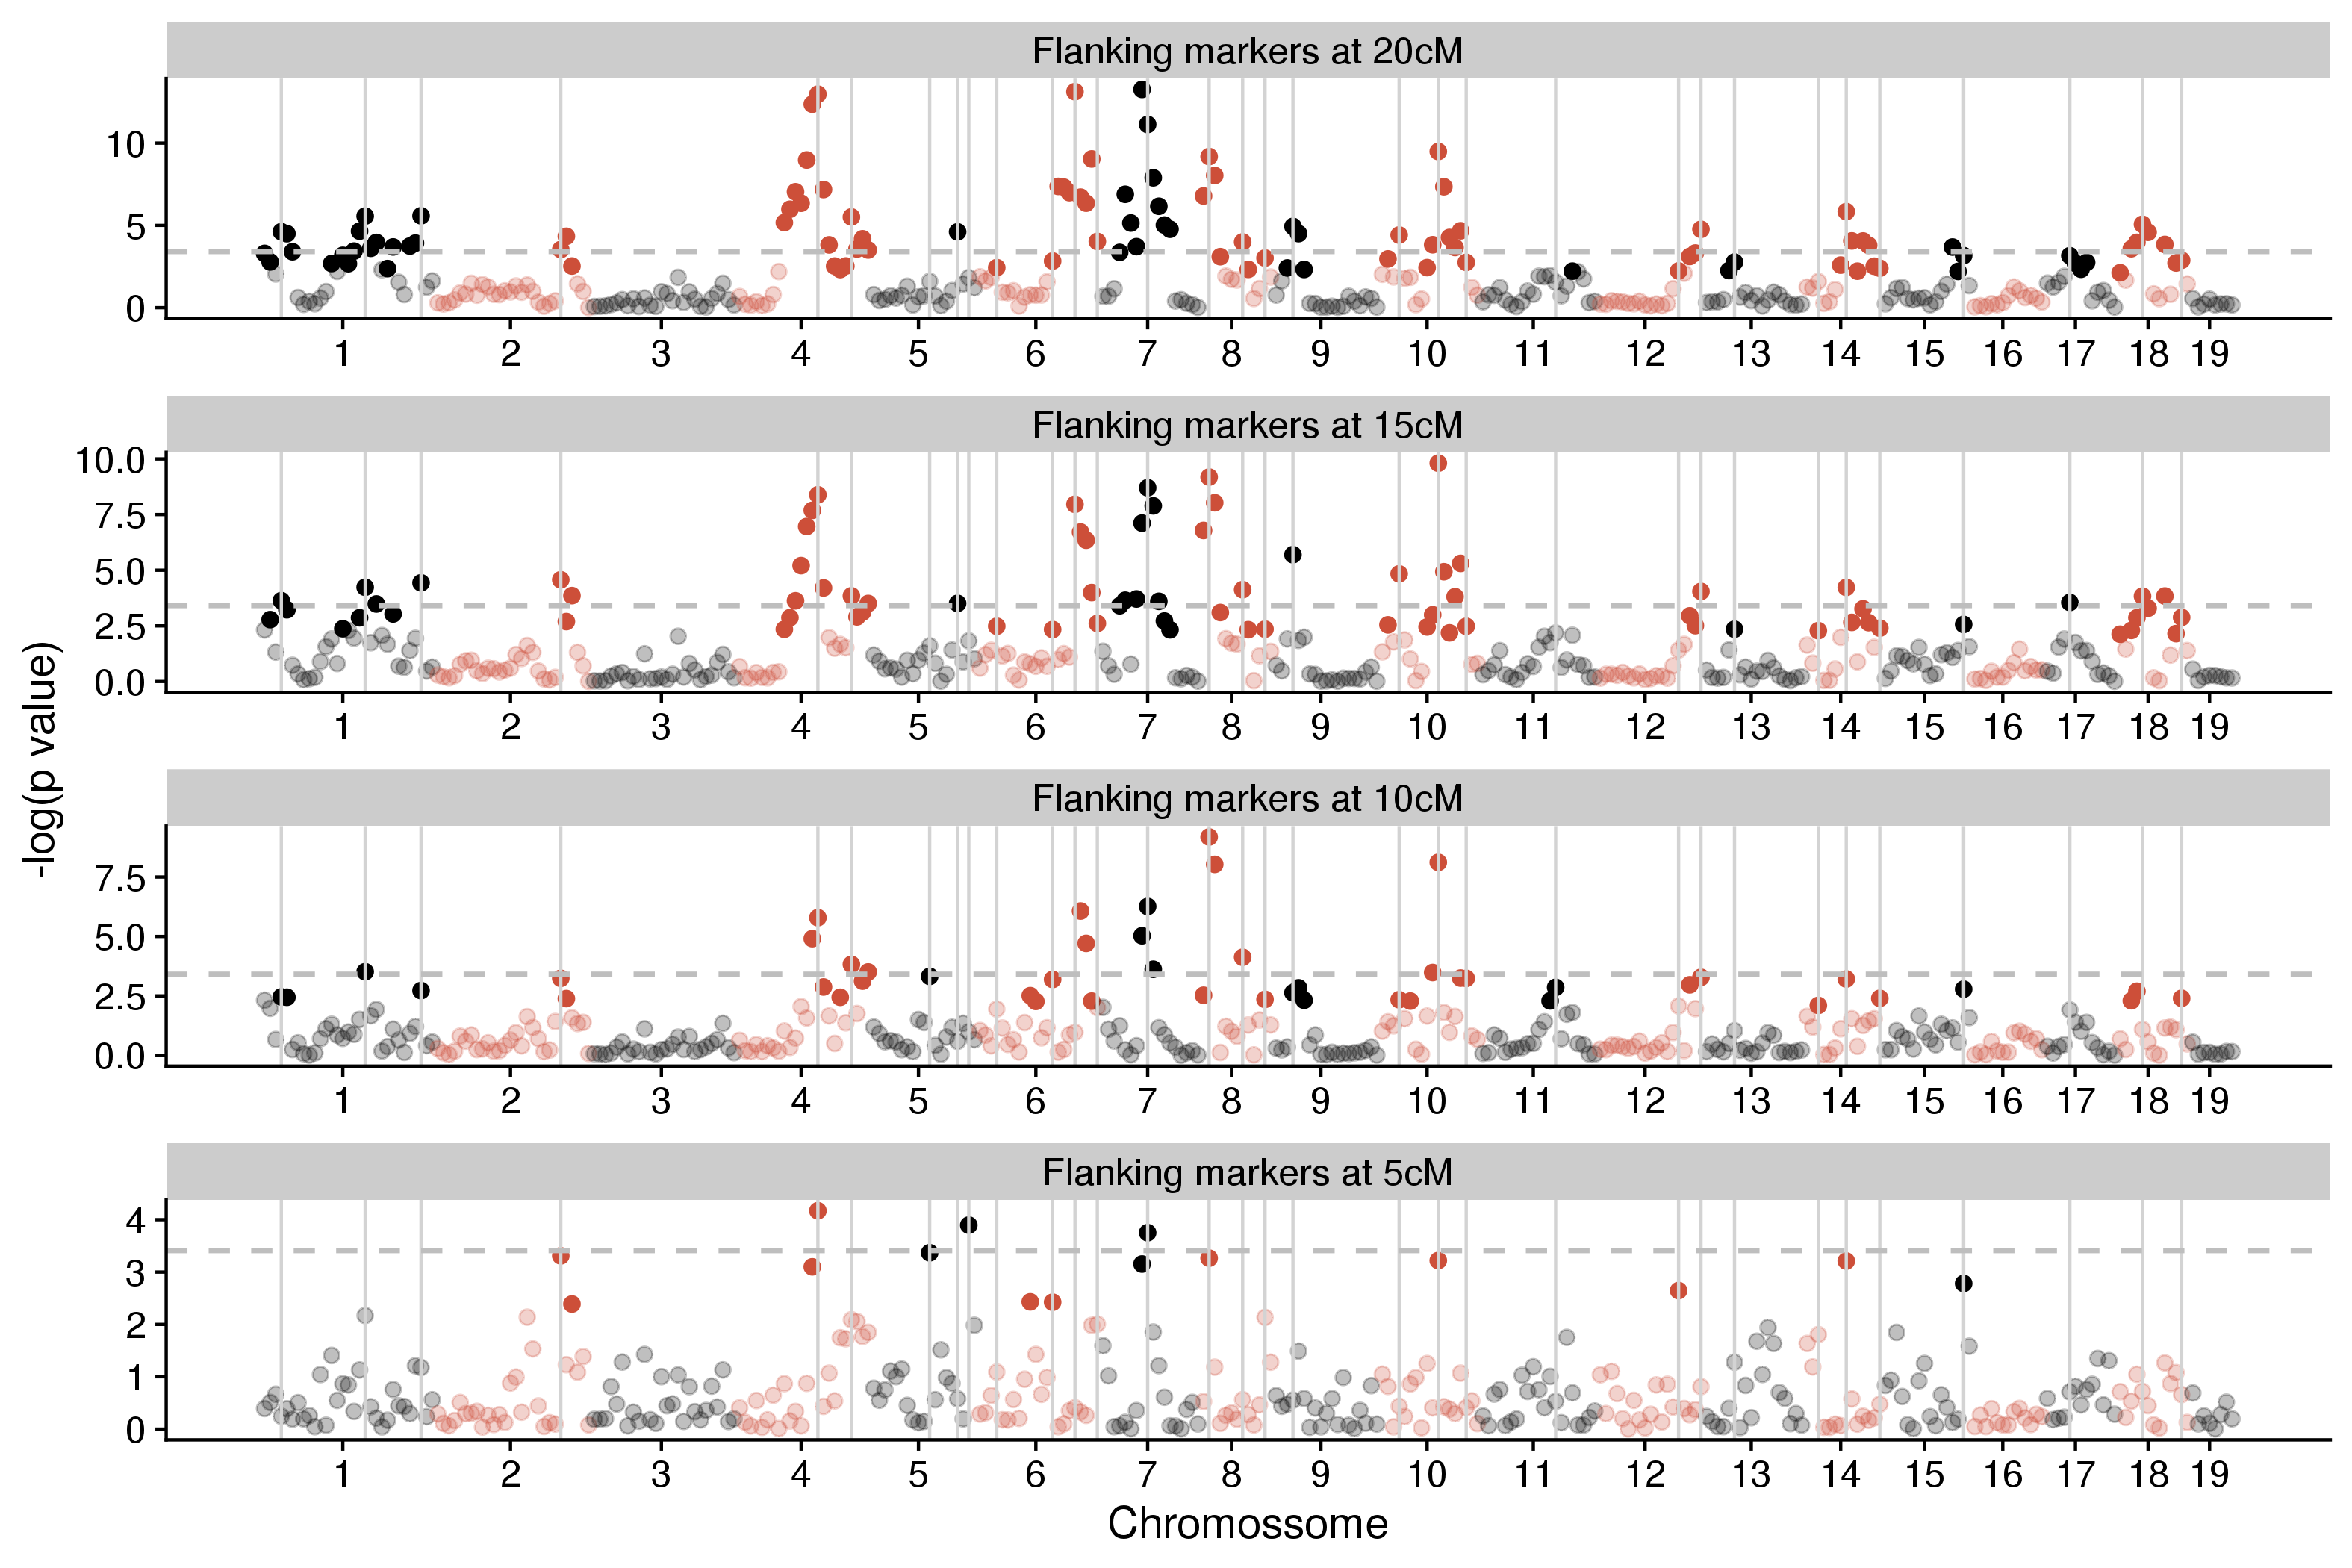
\includegraphics[width=\linewidth]{chapter_JoH-Melo_etal/media/growth_manhattan.png}
\caption[Mapped markers]{Identified makers using interval mapping with various
flanking marker distances. Chosen markers are shown as gray vertical
lines. Significant markers at the chromosome levels are shown in full
color, non significant markers at the chromosome level are translucent,
the dashed line marks the whole genome significance threshold.
Chromosomes are shown in alternating
colors.}
\label{fig:joh:manhatan}
\end{figure}

\begin{figure}
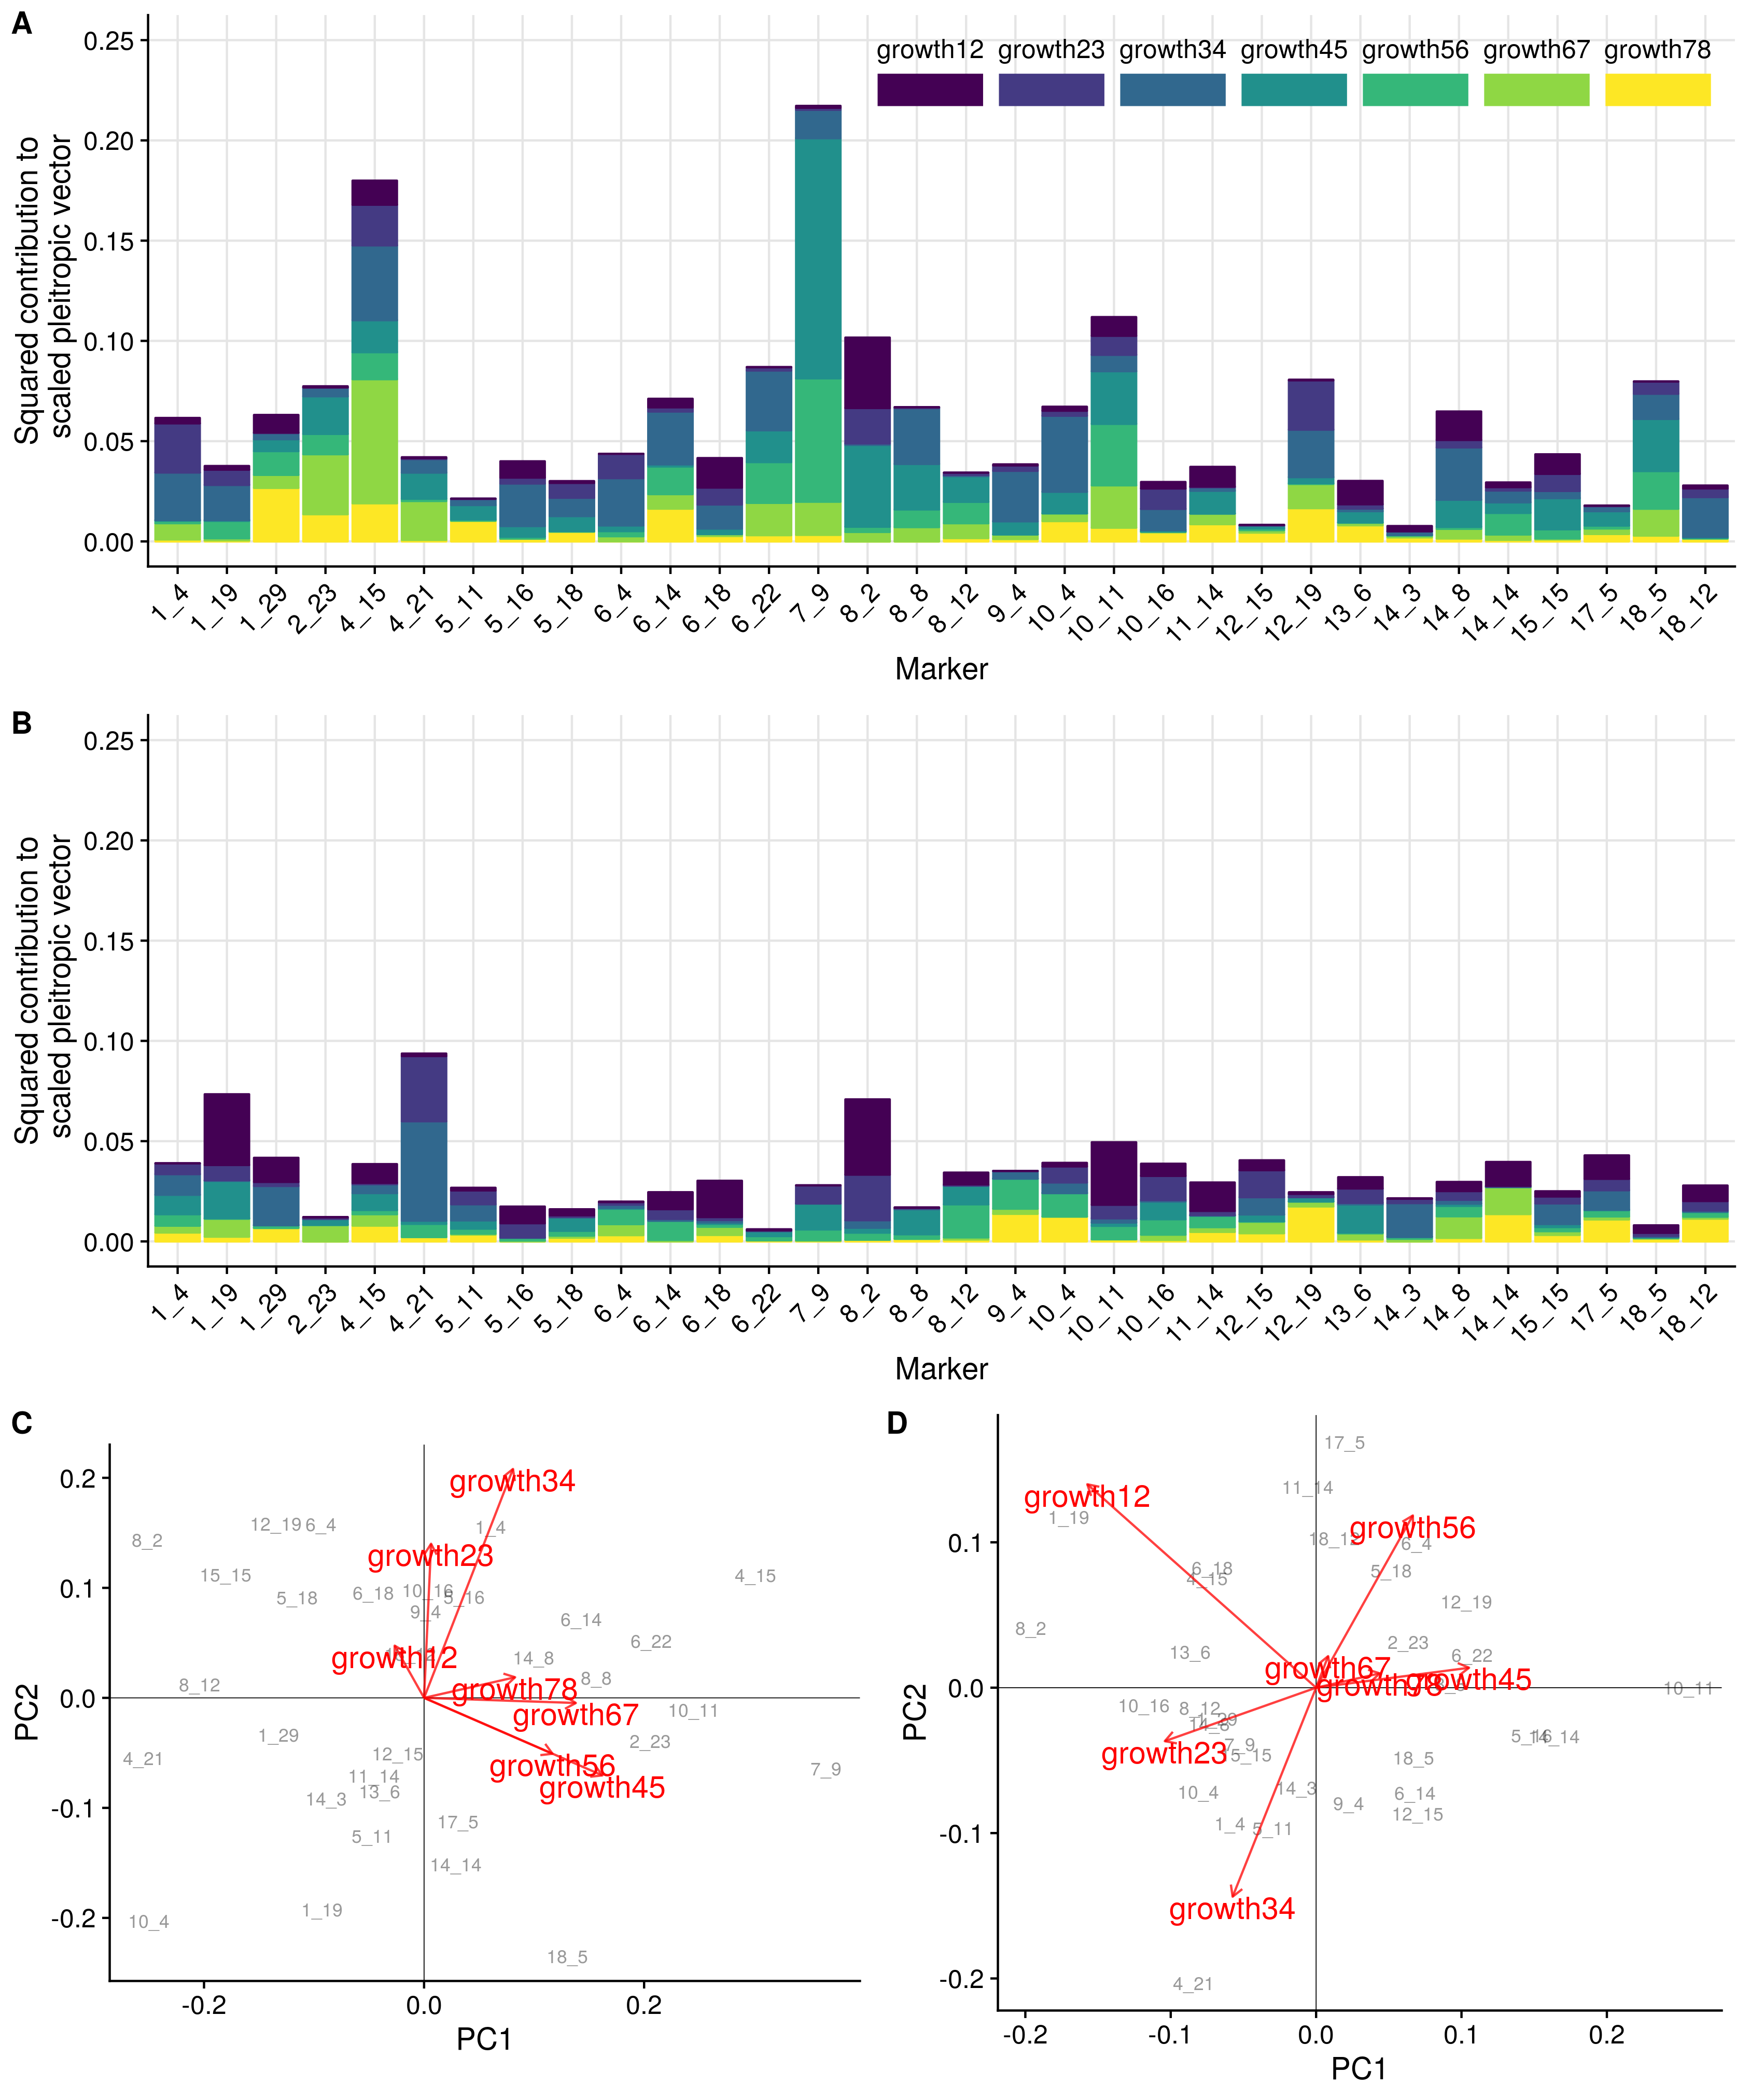
\includegraphics[width=\linewidth]{chapter_JoH-Melo_etal/media/growth_pleiotropic_partition_ad_dm.png}
\caption[Pleiotropic effects of identified markers]{Pleiotropic effects of identified markers. (A) additive
and (B) dominance contributions of the trait components to the final
length of the pleiotropic vector. All trait contributions are scaled to
trait standard deviation and are comparable. (C) additive and (D)
(dominance): PCA of marker effects, arrows represent trait loadings in
PC 1 and 2, marker IDs in grey are marker scores in PC 1 and 2. Markers
are coded as chromosome and marker within chromosome, see SI for genomic
position.}
\label{fig:joh:pleiopart}
\end{figure}

\begin{figure}
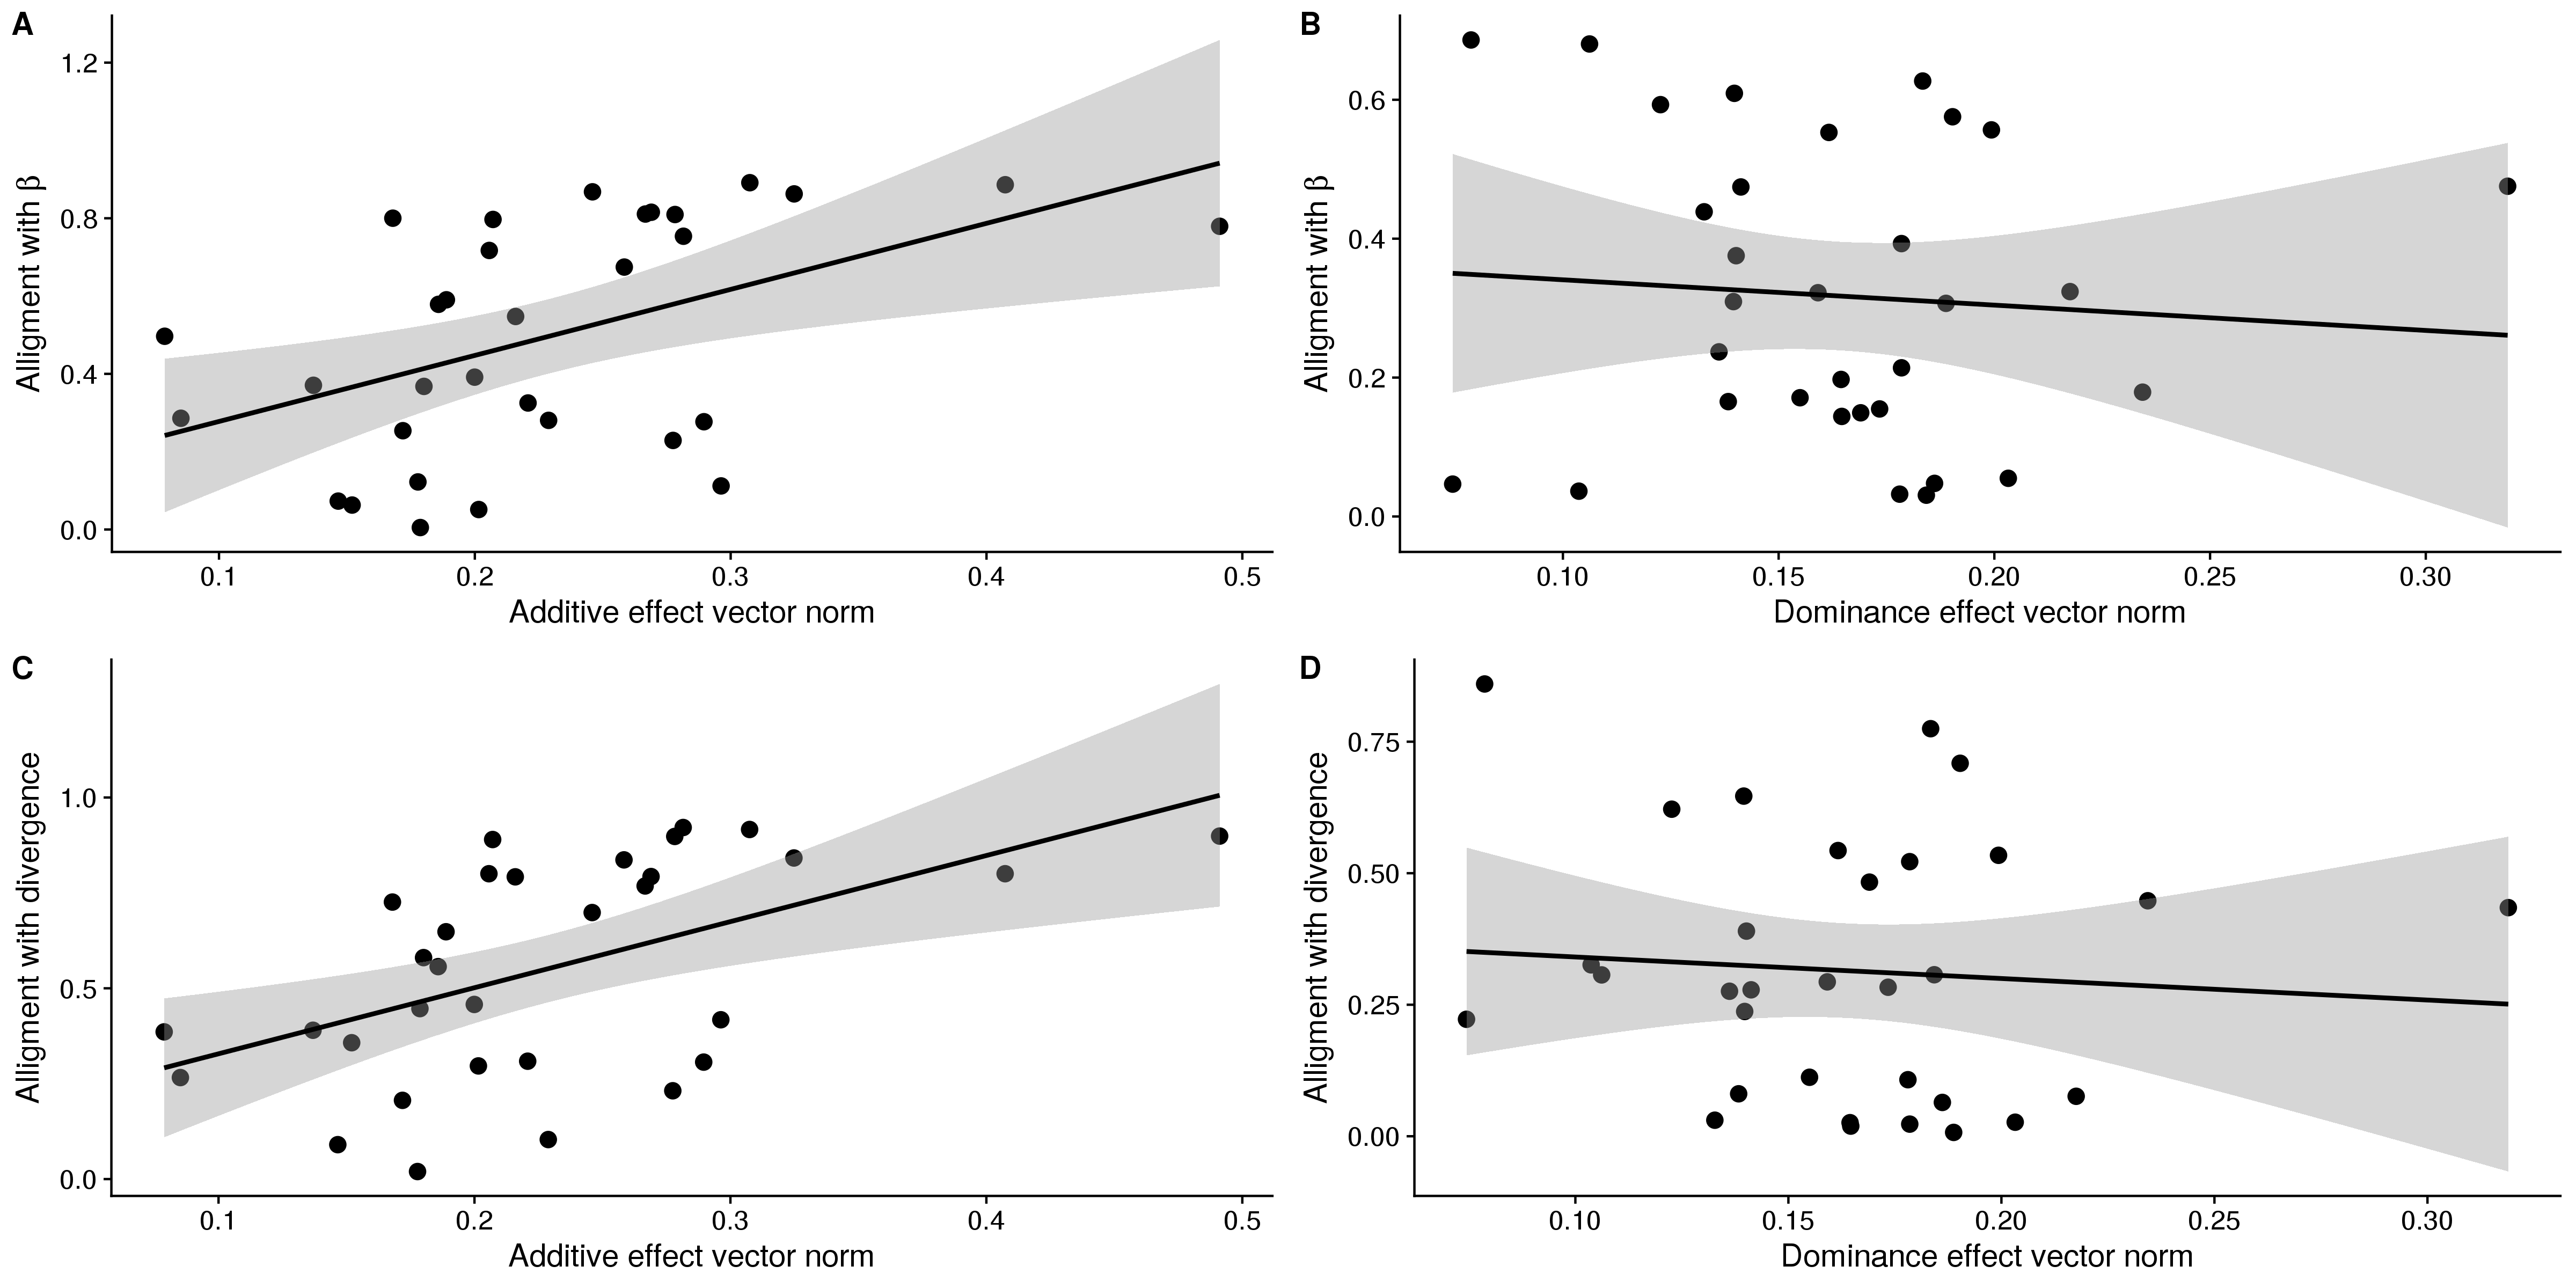
\includegraphics[width=\linewidth]{chapter_JoH-Melo_etal/media/growth_effect_aligment_regressions.png}
\caption[Size and alignment for chosen markers]{Size and alignment for chosen markers. Pleiotropic
effect vector alignment with selection and divergence between founders.
Panels A and B show the relation between pleiotropic effect vector norm and alignment
to estimated selection gradient ($\beta$), while panels C and D show the relation between
pleiotropic effect vector norm and alignment to phenotypic divergence. A)
and C) additive effects; B) and D) dominance effects.}
\label{fig:joh:alignment}
\end{figure}

\subsection{Genome Prediction}

Genome prediction produces pleiotropic effect vectors for all markers
(Fig.~\ref{fig:joh:pleiopartGP}). We again see a widespread pattern of pleiotropy, but less so
than in the mapped effects, as several of the large effect vectors have
effects in only one or two traits. This is especially evident in the
dominance effects. The PCA plot of marker effects confirms this, as the
first two PCs are not related to early and late growth, as in the mapped
markers, but combinations of single trait effects. We can also see the
pattern of linkage affecting the pleiotropic vectors, as larger effects
are often clustered and similar, suggesting that the regularization
shrinkage prior was unable to pick a single marker as the best position
for the effect, spreading the putative QTL over several neighboring
markers (this is a known limitation of this type of sparse regression,
see \textcite{Piironen2017-ih}). We can also see the pattern that larger additive effect vectors
are more aligned with phenotypic divergence. Small effects, which where
shrunken toward zero by the horseshoe prior, are essentially pointing in
random directions, while larger additive vectors are more aligned with
divergence and selection (alignment with divergence, slope = 2.42,
\emph{p} \textless{} 0.001; alignment with selection gradient, slope =
1.75, \emph{p} \textless{} 0.001, Fig.~\ref{fig:joh:alignmentGP}A and C). Dominance vectors
again don't have any pattern between magnitude and alignment (alignment
with divergence, slope = -2.01, \emph{p} = 0.09; alignment with
selection gradient, slope = -2.14, \emph{p} = 0.08, Fig.~\ref{fig:joh:alignmentGP}B and D).

\begin{figure}
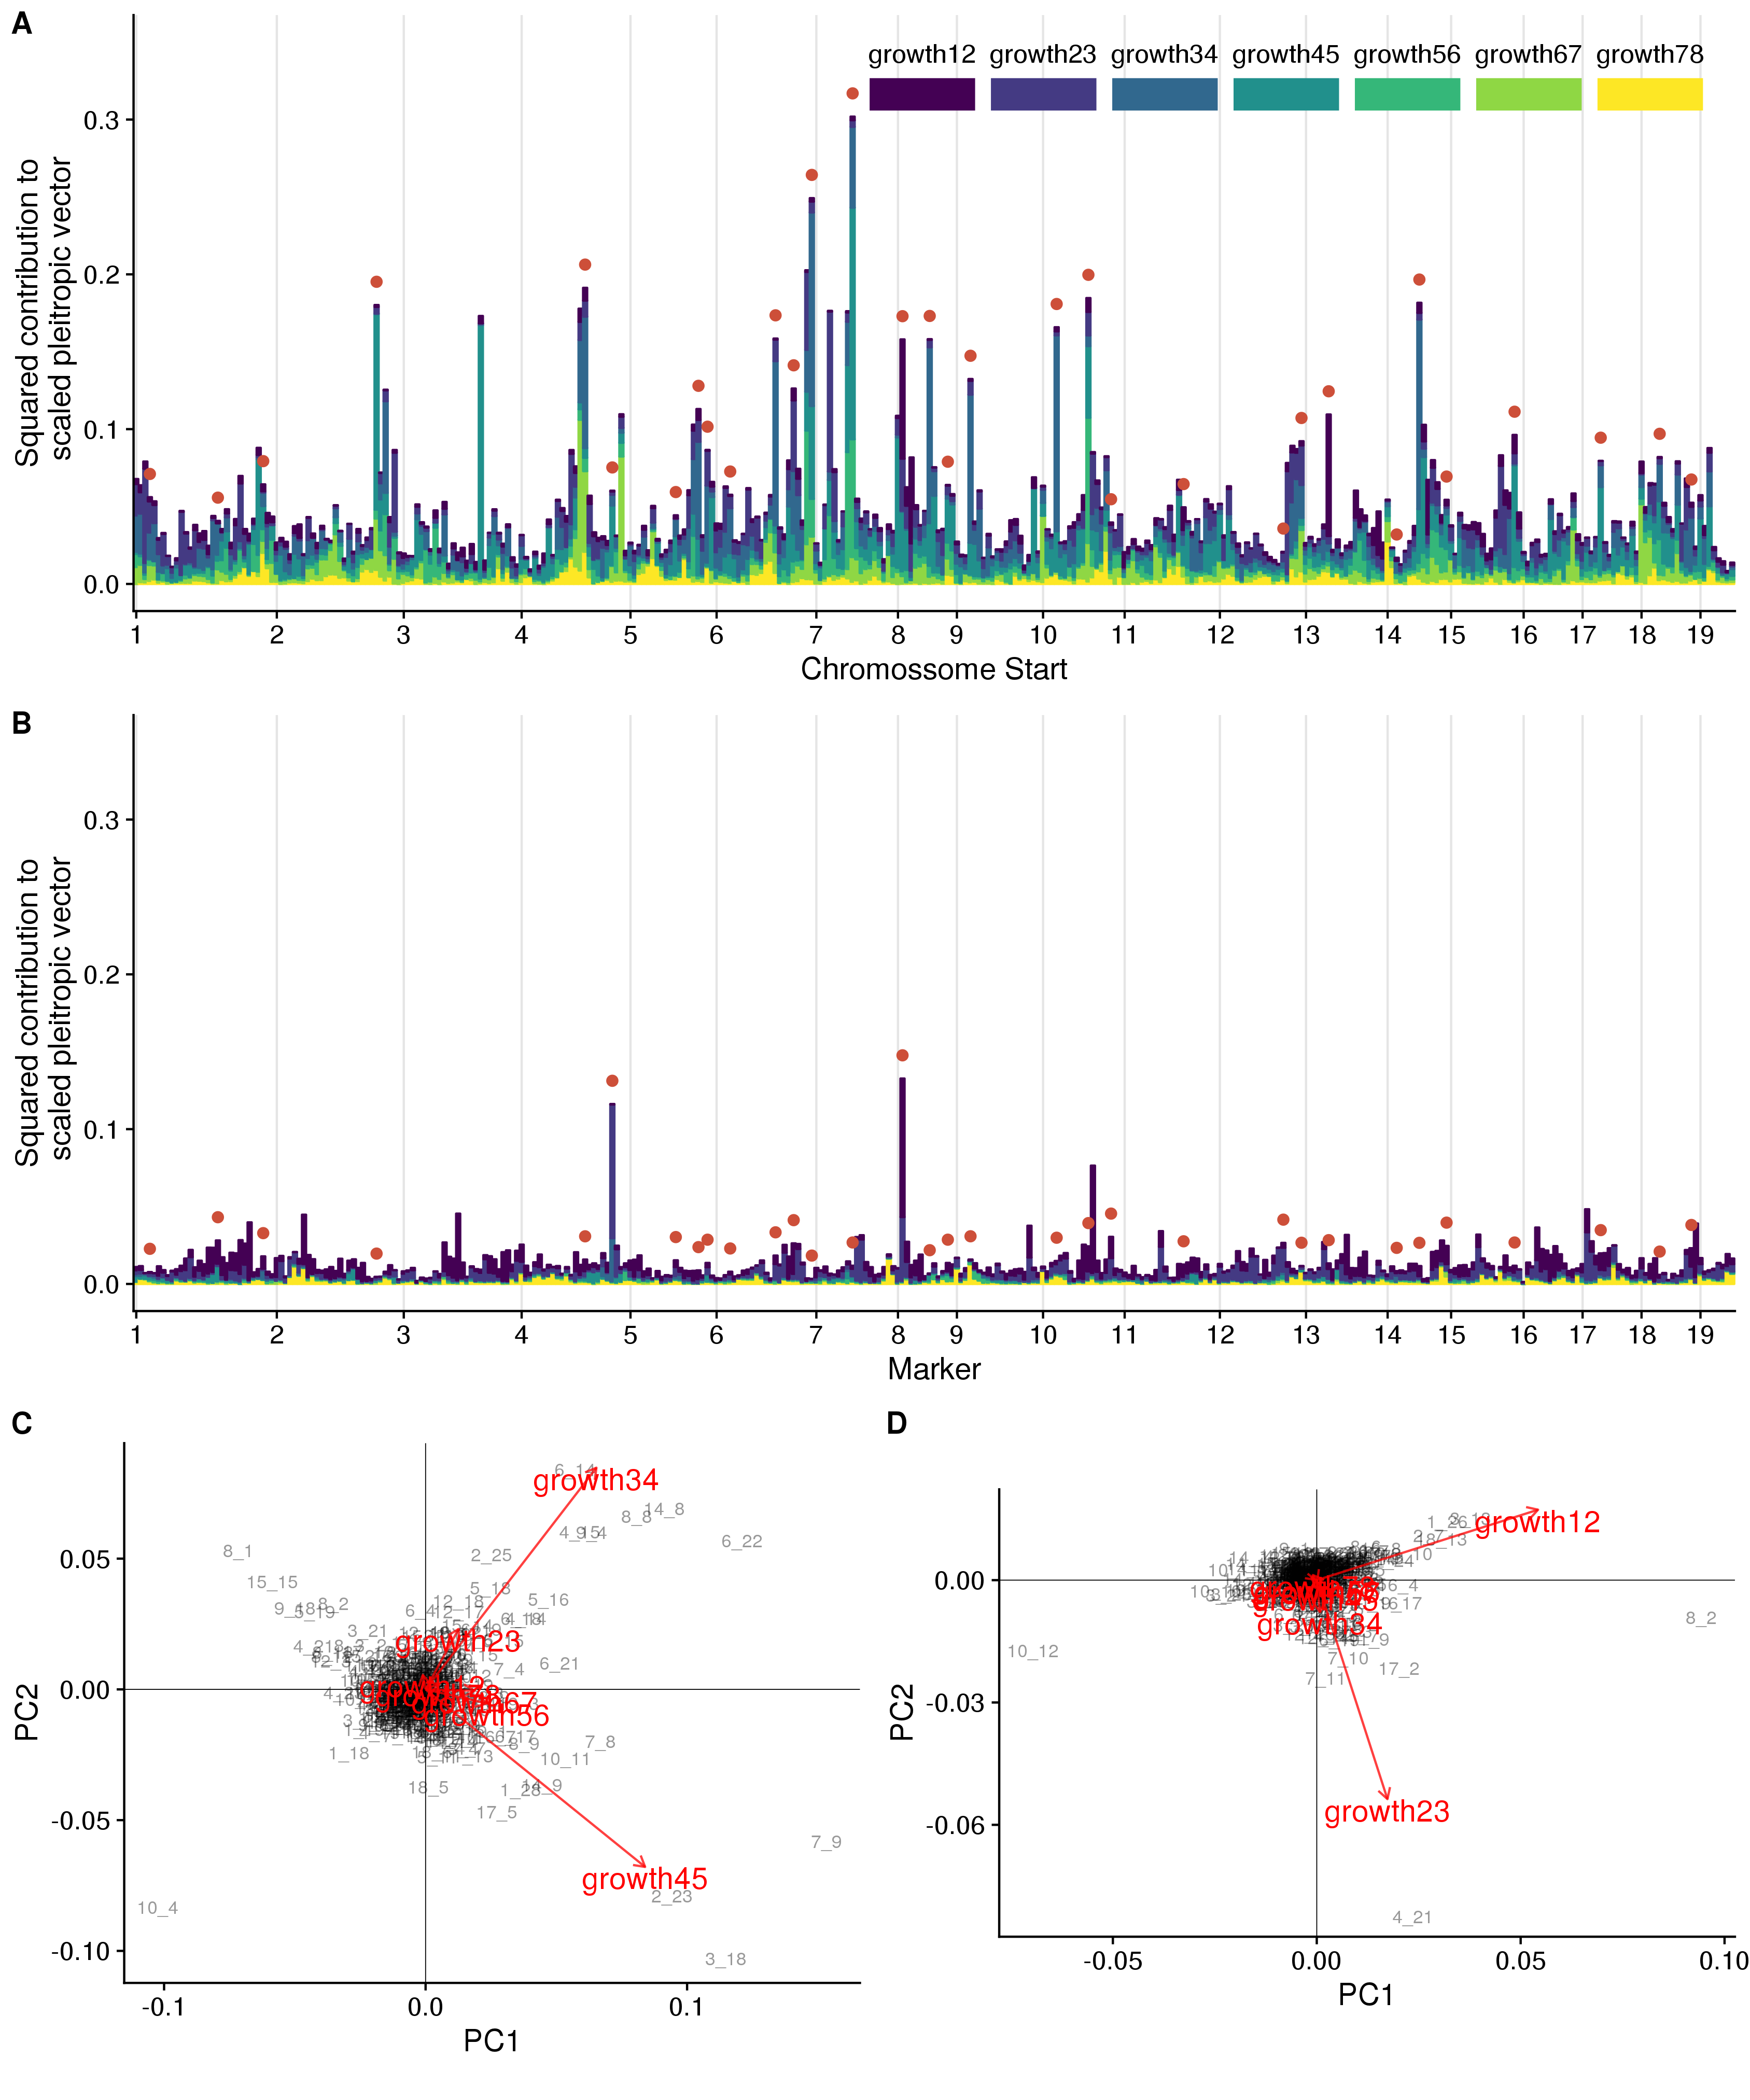
\includegraphics[width=\linewidth]{chapter_JoH-Melo_etal/media/growth_pleiotropic_partition_ad_dm_GP.png}
\caption[Pleiotropic effects of all markers]{Regularized pleiotropic effects of all markers. (A) additive
and (B) dominance contributions of the trait components to the final
length of the pleiotropic vector. Significant markers in the QTL mapping are marked by
the red dots. All trait contributions are scaled to trait standard
deviation and are comparable. (C) additive and (D) dominance PCA of marker effects, arrows
represent trait loadings in PC1 and PC2, marker IDs in gray are marker
scores in PC 1 and 2.}
\label{fig:joh:pleiopartGP}
\end{figure}

\begin{figure}
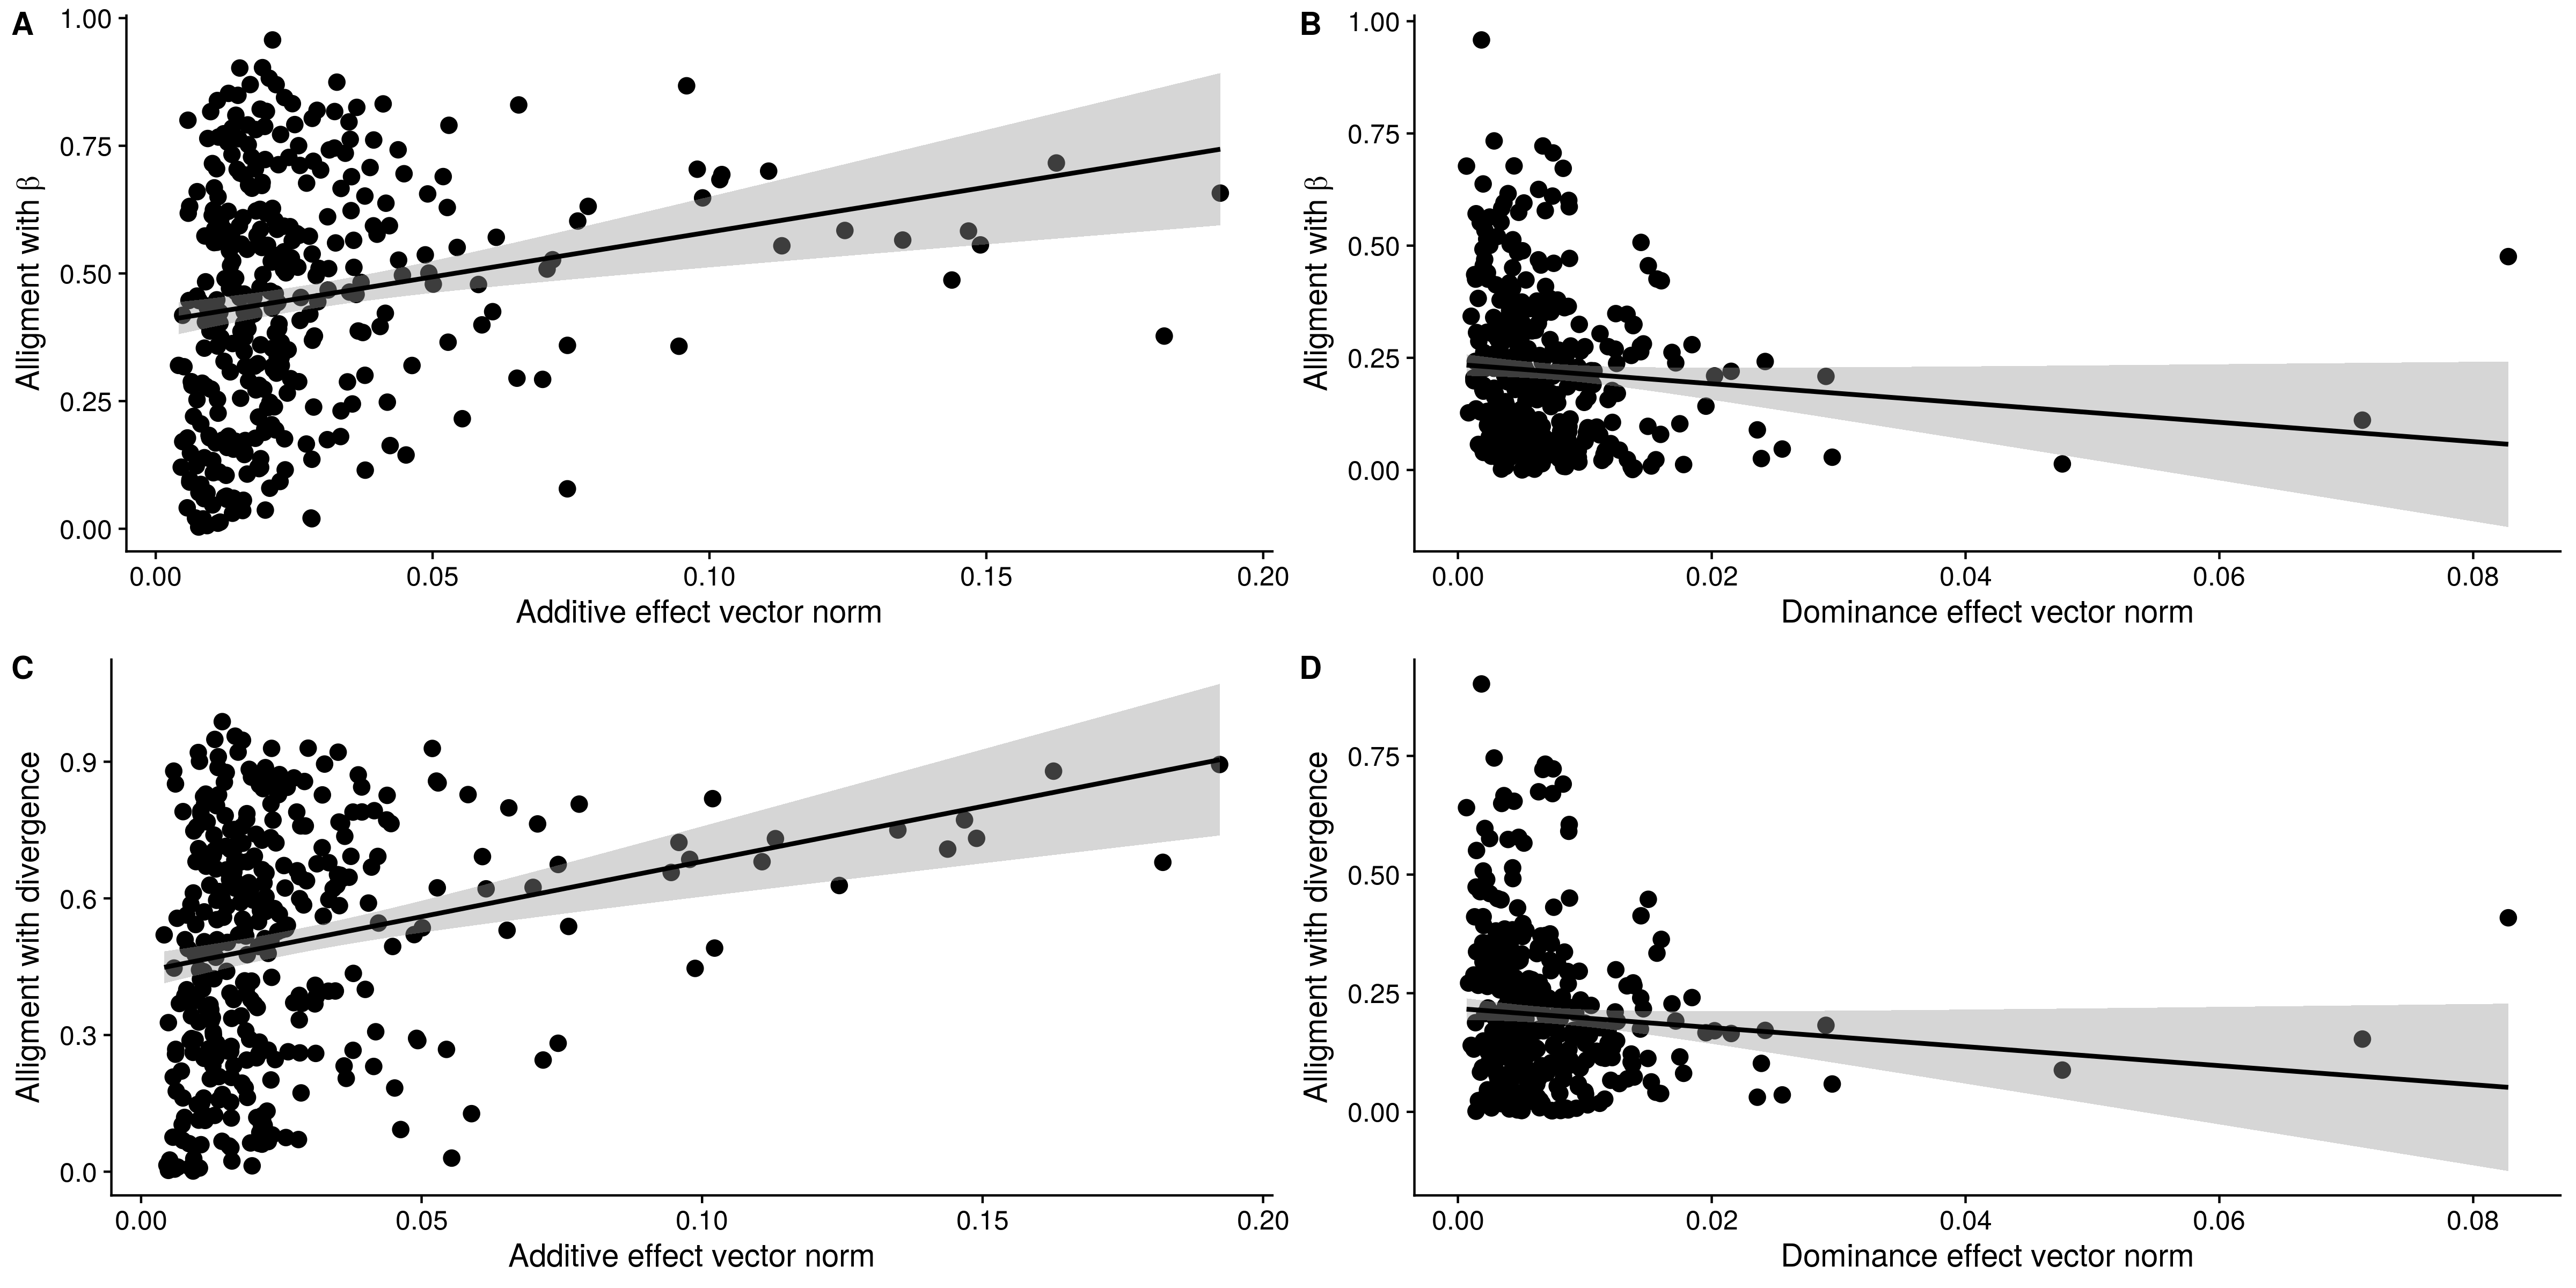
\includegraphics[width=\linewidth]{chapter_JoH-Melo_etal/media/growth_effect_aligment_regressions_GP.png}
\caption[Pleiotropic effect vector alignment]{Regularized pleiotropic effect vector alignment with selection
gradient and divergence between founders. Panels A and B show the relation between regularized pleiotropic effect vector norm and alignment to estimated selection gradient ($\beta$), while panels C and D show the relation between
pleiotropic effect vector norm and alignment to phenotypic divergence. A)
and C) additive effects; B) and D) dominance effects.}
\label{fig:joh:alignmentGP}
\end{figure}

\subsection{Ancestral predictions}

Both regression models do well at predicting the phenotypes of the
founder strains using only genetic effects estimated from the
F\textsubscript{3} generation (Fig.~\ref{fig:joh:ancestral}). The genome prediction method is
slightly better on the average prediction, but most ancestral growth
periods are inside the posterior distribution (grey lines) for both
models. First week of growth is somewhat anomalous in that the
F\textsubscript{3} generation is not intermediate to the two founders,
possibly due to environmental effects, and so the prediction is poor.
Growth in week 4 in the Large strain is larger than predicted from the
F\textsubscript{3} genetic effects, suggesting either non-detected
effects in the F\textsubscript{3} or some other non-additive genetic or
environmental effects. The same applies to the week 7 growth, where both
Large and Small strains are more different from the F\textsubscript{3}
then expected from the F\textsubscript{3} additive effects.

\begin{figure}
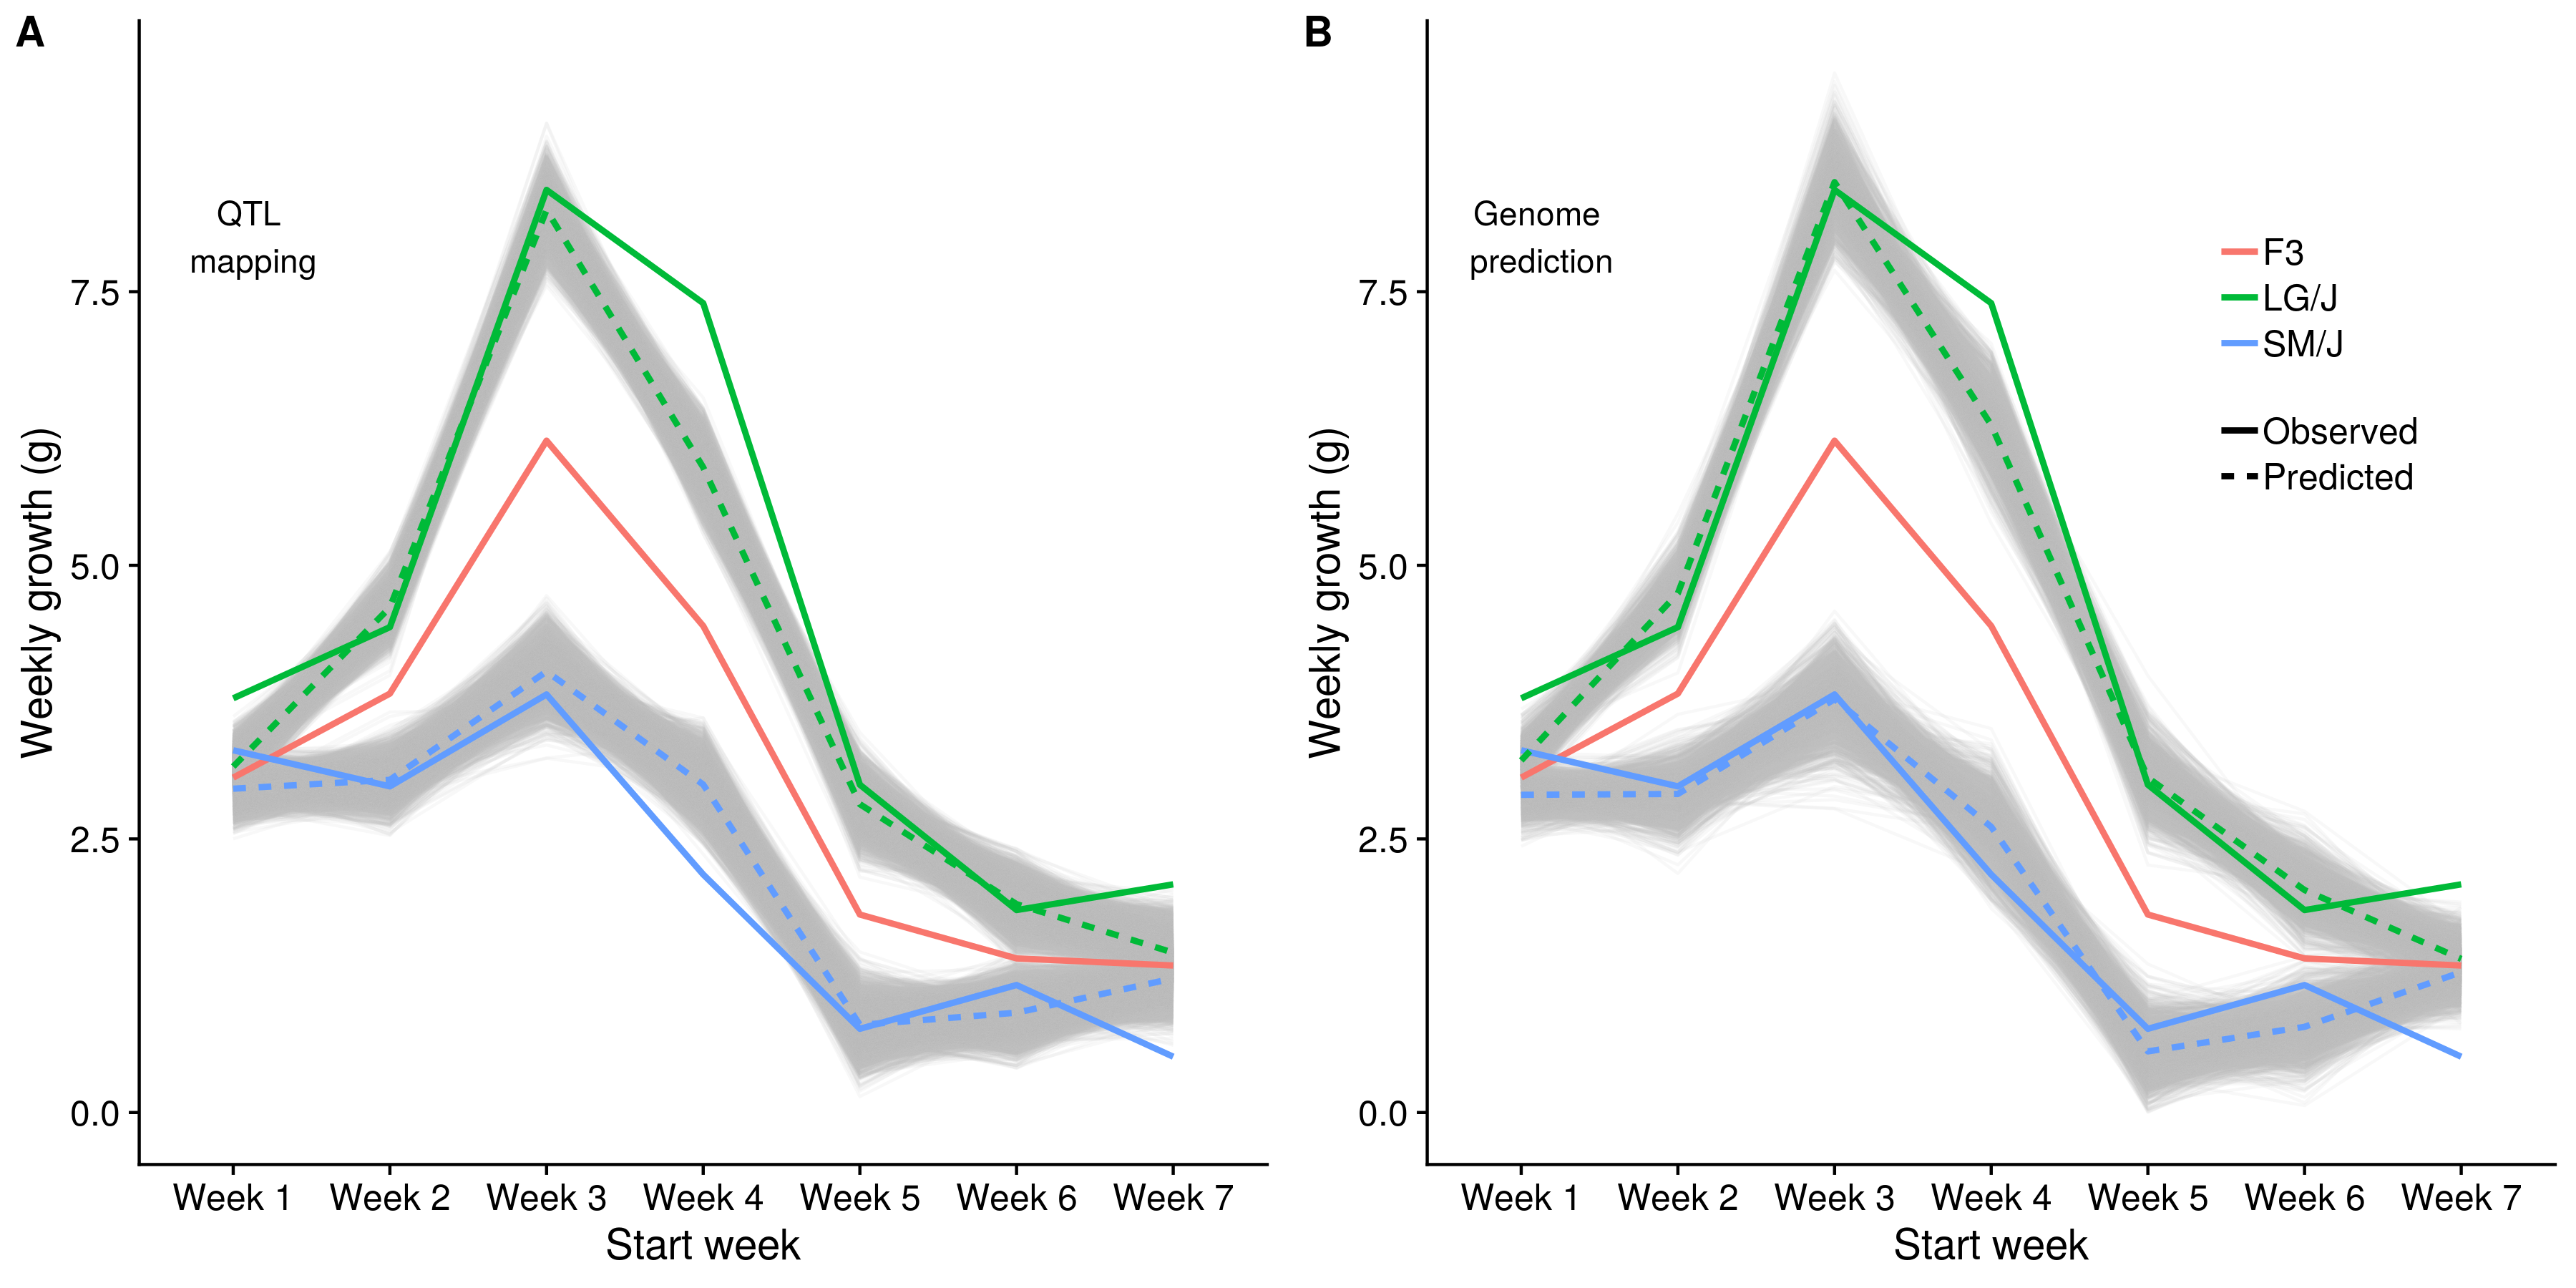
\includegraphics[width=\linewidth]{chapter_JoH-Melo_etal/media/growth_LG_SM_F3_predictions.png}
\caption[Ancestral predictions from additive effects]{Ancestral predictions from additive effects.
Predictions of the ancestral growth curves using additive effects
estimated in the F\textsubscript{3} generation. Solid lines are the
observed growth curves, dashed lines the predicted growth curves from
the two models. (A) QTL mapping of significant markers, (B) Genome
prediction using all markers. Grey lines represent the posterior
distribution of ancestral predictions derived from the Bayesian effect
estimates.}
\label{fig:joh:ancestral}
\end{figure}

\subsection{Covariance matrix predictions}

Genetic correlation matrices estimated from the pleiotropic effects from the
mapped markers are broadly similar to the family level full-sib genetic matrix
estimated from the mixed model fit. We can see the same strong correlation
between late growth, and the positive correlation between weeks 2 and 3. The
negative correlation between weeks 2 and 4 is present, but much smaller in
magnitude in the QTL estimated matrix. The smallest correlations are between
the early and late traits. Regressing the full-sib genetic matrix onto the
genetic covariances predicted from the mapped markers (given by the sum of
half the additive genetic matrix with one quarter of the dominance genetic
matrix) reveals that the observed covariances are in general much larger than
the predicted ones, but the pattern of covariances is similar (intercept =
-0.01, slope = 2.43, \emph{p} \textless{} 0.001). The outliers in the
regression are the negative covariance between weeks 2 and 4 and the much
larger observed variance in week 4. This is not surprising, since the full-sib
genetic includes other sources of covariation, like maternal and common
environmental effects. The genome prediction fared much worse, predicting
variances and covariances close to zero for almost all traits (see
Fig.~\ref{fig:joh:covGP}). Matrix comparisons can be seen in
Table~\ref{joh:matcompare}. The most similar matrices are the QTL mapping
maker genetic matrix, followed by the QTL mapping marker additive genetic
matrix. Both show high similarities in Random Skewers, Mantel matrix
correlation, and a high proportion of shared subspace. The dominance matrix
shows a relatively low matrix correlation and the lowest Krzanowski shared
sub-space correlation, suggesting it is different in structure to the full-sib
genetic matrix. Genome prediction matrices have very low, non-significant
Mantel correlation values, reflecting the poor estimate of the G-matrix
correlations. Random Skewers comparisons are all relatively high and
significant, with the exception of the genome prediction dominance matrix.
This can be due to a relatively similar first principal component in all
matrices.

\begin{figure}
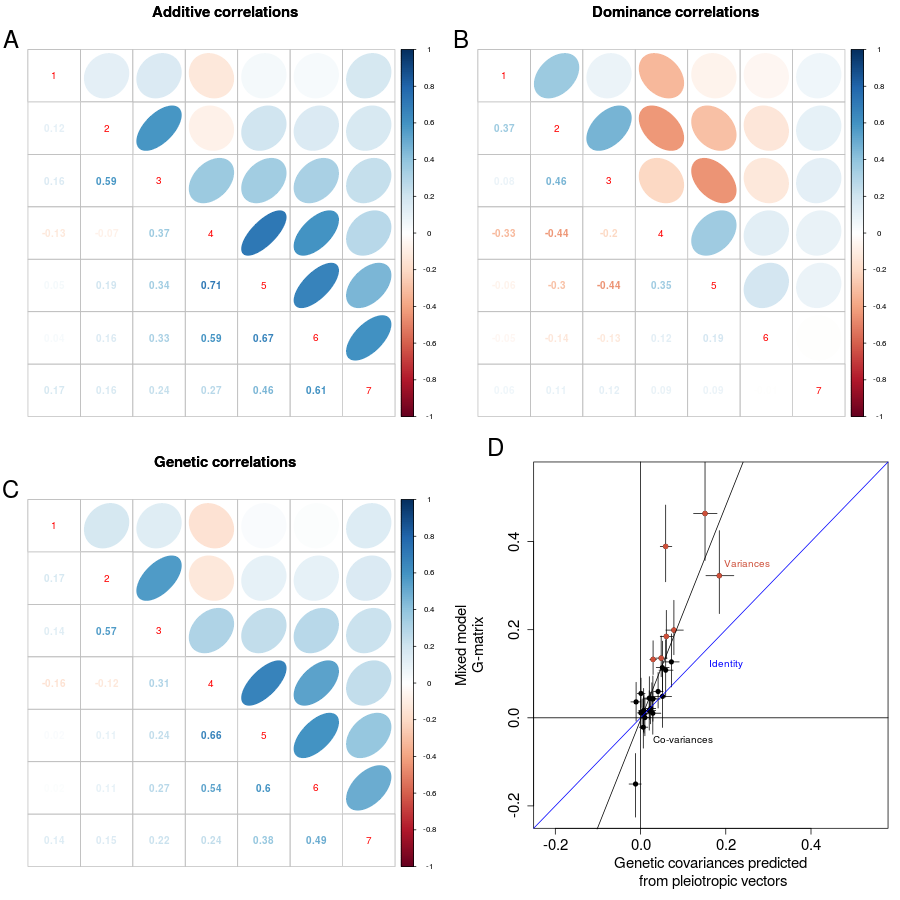
\includegraphics[width=\linewidth]{chapter_JoH-Melo_etal/media/growth_cov_prediction_composite.png}
\caption[Additive, dominance and genetic matrices]{Additive, dominance and genetic matrices. Estimated
correlation matrices from QTL mapping marker effects. (A) additive, \textbf{G}, (B)
dominance, \textbf{D} (C) Genetic, ½ \textbf{G} + ¼ \textbf{D}. (D) Regression of
genetic variances and covariances estimated from full-sib mixed model
and estimated from markers. Error bars represent 95\% posterior
credibility intervals. Marker-estimated covariances are about half of observed
covariances.}
\label{fig:joh:cov}
\end{figure}

\begin{table}[htbp]
	\caption[Matrix comparisons of the QTL and Genome
	prediction matrices]{Matrix comparisons of the QTL mapping and Genome
	prediction marker based matrices with the estimated full-sib genetic
	via Random Skewers, Mantel correlation and Krzanowski shared subspace
	correlation.}
	\vspace{1em}
	\centering
	\begin{tabular}{l|ccc}
	\toprule
	& \multicolumn{3}{c}{Similarity to Family full-sib genetic matrix} \\
\cline{2-4}
Matrix & \multirow{2}{*}{Random Skewers} & Mantel  & Krzanowski  \\
& & correlation & correlation \\
\midrule
QTL-mapping marker  & \multirow{2}{*}{0.872 (p \textless{} 0.001)} & \multirow{2}{*}{0.69 (p \textless{} 0.001)} & \multirow{2}{*}{0.86} \\
additive genetic matrix & & & \\
\cline{1-1}
QTL-mapping marker & \multirow{2}{*}{0.85 (p = 0.005)} & \multirow{2}{*}{0.49 (p = 0.01)} & \multirow{2}{*}{0.62} \\
 dominance genetic matrix & & & \\
\cline{1-1}
QTL-mapping marker  & \multirow{2}{*}{0.89 (p \textless{} 0.001)} & \multirow{2}{*}{0.70 (p = 0.002)} & \multirow{2}{*}{0.86} \\
genetic matrix (½ G + ¼ D) & & & \\
\cline{1-1}
Genome prediction marker & \multirow{2}{*}{0.82 (p = 0.007)} & \multirow{2}{*}{0.09 (p = 0.28)} & \multirow{2}{*}{0.78} \\
 additive genetic matrix  & & & \\
\cline{1-1}
Genome prediction marker & \multirow{2}{*}{0.6 (p = 0.057)} & \multirow{2}{*}{0.20 (p = 0.16)} & \multirow{2}{*}{0.40} \\
 dominance genetic matrix & & & \\
\cline{1-1}
Genome prediction marker & \multirow{2}{*}{0.83 (p = 0.002)} & \multirow{2}{*}{0.12 (p = 0.29)} & \multirow{2}{*}{0.77} \\
genetic matrix (½ G + ¼ D)  & & & \\
\bottomrule
	\end{tabular}
	\label{joh:matcompare}
\end{table}

\section{Discussion}

The interaction between selection and multivariate covariation is a central
part of our understanding of evolution. Even simple selection regimes can
produce complex multivariate responses due to cascading developmental effects
and genetic constraints. Here, we use a cross between two artificially
selected lines of mice to investigate the genetic architecture of the
multivariate response due to artificial selection. The target of selection in
both lines was individual final weight, in opposite directions, and we use the
various phases of growth as a model of a multivariate trait altered by
selection. Using multivariate QTL mapping and genomic regression, we were able
to map loci involved in the variation of growth and to simultaneously estimate
vectors of genetic effects responsible for the variation in growth. Combining
these effect vectors with quantitative genetics theory, we were able to
directly link the pattern of pleiotropy and the genetic covariation of these
traits.

As expected by the behavior of the phenotypes in the cross
\parencite{Cheverud1996-fm}, most of the divergence between Large and Small is
due to additive effects. The mean additive effect vector is practically
collinear with the direction of divergence between lines, and we see a
relation between the total size of the additive effects and the alignment with
selection and divergence. This relation between alignment and size reflects
the effect of selection removing large effects in other directions, that is,
the larger the pleiotropic effect the more it must conform to the direction of
selection in order to be maintained, while smaller effects can be less aligned
with selection and still contribute to the divergence between lines. This
clear alignment is absent from the dominance effect vectors, as the mean
dominance vector has low correlation with the phenotypic divergence and the
direction of selection, and the size of the individual marker effects also has
no bearing on their alignment to divergence and selection. Dominance vectors
are not expected to contribute to the phenotypic divergence, since they are an
interaction effect between alleles from the two founder lines, and so are only
present in the crosses. These relations between effect size and alignment are
present in both QTL mapping and genome prediction estimates of the additive
and dominance effect vectors, but in the genome prediction the relations are
much less clear when we look at the very small vectors. These small effect
vectors are distributed in all directions but have very small norms (which is
a measure of the overall effect of the locus across traits). Presumably, this
is indicative that they have negligible effect on the phenotype and are being
shrunk to zero by the sparse regression priors, and so the individual vector
directions are essentially random.

Ancestral predictions using QTL mapping is surprisingly accurate, and most of
the ancestral traits are within the posterior distribution of ancestral
estimates, even though we are using only a small number of large effect QTL in
the prediction model. The genome prediction analysis using sparse regression,
on the other hand, is potentially including a number of small effects that do
not meet a significance threshold, and so are excluded from the QTL mapping
analysis. The inclusion of these many small effects have been proposed as a
solution to the missing heritability problem \parencite{Bloom2013-xc, Boyle2017-re}, and
modern sparse regression and genomic prediction methods provide a promising
framework for working with high density marker data sets \parencite{Pong-Wong2014-vj}. 
Indeed, the sparse regression produces very good out-of-sample
predictive performance when used to predict the phenotypes of the founder
lines (Fig.~\ref{fig:joh:ancestral}). Mapping could also be done in this
sparse regression framework using variable selection, and the model displays
reasonable agreement with the QTL mapping, producing large effect estimates
that are close to the detected QTL (Fig.~\ref{fig:joh:pleiopartGP}).
Furthermore, our analysis was done in standard generic Bayesian model fitting
software (admittedly this was only possible since our maker data set is
relatively low density, but further advances in general statistical software
should make using similar approaches in larger datasets possible). QTL
mapping, on the other hand, provides us with a small set of interpretable
pleiotropic vectors, which capture the modular aspects of early and late
development, and can be used to understand the pattern of covariation that we
see in the G-matrix. Although the inclusion of all the marker helps with the
ancestral prediction and uses effects that are ignored by the QTL mapping,
using all of the markers for the estimation of expected covariances seems to
be much more susceptible to noise introduced by small effect markers than the
mean ancestral predictions, and the marker estimated variances and covariances
using genome prediction are all close to zero. Some sort of variable selection
would be necessary to make this estimate reliable using the genome prediction
estimates. We do not pursue this further, but presumably even gradual removal
of small effects would improve this estimate.

Using the pleiotropic effect vectors estimated in the QTL mapping analysis and
quantitative genetics theory \parencite{Kelly2009-bj}, we were able to
construct expected additive and dominance genetic covariance matrices. The
additive marker matrix is broadly similar to the observed full-sib genetic
matrix, with strong positive correlations between the late traits, a strong
correlation between weeks 2 and 3, and weaker correlations between early and
late traits. The dominance matrix is different, with weak positive
correlations within early and late traits and negative correlations between
them. This clean separation between additive and dominance components of the
G-matrix is difficult to achieve using only breeding experiments, and
underscores how different these genetic effects can potentially be. The
difference in the patterns of additive and dominance covariation suggests that
these patterns have considerable latitude to vary and do not arise from a
fundamental property of the system. If all gene effects on growth were
constrained by some set of developmental pathways, we would expect all sources
of genetic covariation to share a similar pattern, reflecting the
developmental constraints. (For example, a trade-off could restrict a locus
with positive effects on trait A to have negative effects on trait B
regardless of the effects being additive or dominant). The genetic matrix,
composed of a one half the additive matrix plus one fourth the dominance
matrix is similar to the full-sib matrix, but with smaller variances
throughout. The negative correlations between weeks 2 and 4 is present, but
not significant, in the marker estimated matrix (Fig.~\ref{fig:joh:cov}C).
Given that our maker based estimates does not include several components that
are expected to contribute to the genetic matrix, like shared environment and
maternal effects, it is not surprising that the marker estimated variances are
smaller than the observed genetic covariances. The smaller variances and
covariances in the QTL mapping maker based genetic matrix can also be
attributed to the inclusion of only part of the direct genetic effects, since
only loci with larger effects are used. Nevertheless, the general structure of
the full-sib genetic matrix is captured by the expected covariance due to
pleiotropy and linkage of the mapped loci, as we can see in the high values of
matrix similarity and in Fig.~\ref{fig:joh:cov}. The success in predicting the
pattern covariation directly from pleiotropic effects underscores the
importance of pleiotropy in determining genetic covariation, and suggests that
a relatively small number of medium and large effect loci can be responsible
for a large portion of genetic constraints. Another possibility is that the
distribution of pleiotropic effects is shared between small and large effects,
either due to mutation, selection bias, or both. This shared distribution
would explain why the general pattern of covariation, but not the total
amount, is successfully predicted from a small number of markers.

The distribution of pleiotropic effects in the QTL mapping analysis offers
some insights into the genetic architecture of growth. First, we see that the
full distribution of additive pleiotropic effects spans a modular variational
space, with independent principal components aligned with the two stages of
growth, early and late. This is somewhat unexpected given that the vector of
selection on growth was in the direction of coordinated change in all phases
of growth (Table~\ref{joh:vectors}), either increasing or decreasing the
target of selection, week 9 weight. Given this target of selection, we would
expect the distribution of the additive effects responsible for the divergence
between large and small to be wholly aligned with the coordinated change of
all growth phases, either increasing or decreasing all phases of growth.
Indeed, on average, the additive effects are aligned with divergence, and
large effects more so, but we still maintain a number of pleiotropic vectors
with antagonistic effects in both phases, either increasing early traits and
decreasing late traits or \textit{vice-versa} (markers on the top-left and
bottom-right quadrant of Fig.~\ref{fig:joh:pleiopart}C). The maintenance of
this modular variation in pleiotropic effects could be associated with
developmental or mutational constraints on the additive genetic effects. But,
if this were the case, we might expect the dominance effects, which are not
shaped by selective history of the founders, to have a similar modular
pattern. While the dominance effects PCA does not show the same clear early-late 
separation in orthogonal directions that we see in the additive effects,
the dominance genetic matrix has a different distinction between early and
late, with positive correlations within each phase and negative correlations
between. So perhaps the modular aspect of the genetic effects can manifest in
different ways. Additionally, the variational modularity between early and
late growth that we see in the G-matrix is not only due to markers having
modular effects, restricted to one stage of growth or another (markers close
to the x and y axis in Fig.~\ref{fig:joh:pleiopart}C), but is also due to a
combination of markers that have general effects in both stages (markers along
the main diagonal, in top-right and bottom-left quadrants in
Fig.~\ref{fig:joh:pleiopart}C) or the previously mentioned markers with
antagonist effect in both stages. This reinforces the idea that there are
several genotype-phenotype maps that can generate a modular covariance matrix
\parencite{Pavlicev2011-xm}. However, several studies have found very low
levels of antagonistic pleiotropy and many more modular pleiotropy in
morphological traits \parencite{Leamy1999-dm,Leamy2002-nh,Kenney-Hunt2008-bd},
suggesting that perhaps the specific genetic architecture underlying
modularity could vary depending on the type of trait and on its evolutionary
history.

\enlargethispage{\baselineskip}
The explicit link between genetic effects and covariation is a natural way to
study multivariate evolution, but still rare in the literature
\parencite{Kelly2009-bj}. Using this approach, we were able to decompose the
full-sib genetic matrix into its additive and dominance components. These
components show different patterns of covariation, a consequence of the
differences in the additive and dominance distributions of pleiotropic
effects. Although both classes of genetic effects show some signal of the
division between early and late growth, the modular pattern is much more
obvious in the additive effects. The full-sib covariance matrix, a common
proxy for the additive genetic covariance matrix, is similar to the purely
additive genetic matrix, but could differ more depending on the dominance
component. Furthermore, we were able to accurately reconstruct the ancestral
states in the founders using only the effects estimated in the
F\textsubscript{3} population, and this prediction was improved using all the
markers in a sparse genome prediction model.


\section{Acknowledgments}

We thank Jim Cheverud for insightful discussions that contributed to the
development of this work, Steve Chenoweth for discussions that were critical
for the development of the analytical framework, and Monique Simon for
comments on the manuscript.


\section{Funding}

This work was supported by grants 2014/26262-4 and 2015/21811-2 from the
Fundação de Amparo à Pesquisa do Estado de São Paulo (FAPESP) to D.M.
and 2011/14295-7 and 2013/50402-8 to G.M., grants BB/L002604/1 and
BB/M01035X/1 from the U.K. Biotechnology and Biological Sciences
Research Council (BBSRC) to J.B.W. and support from the University of
Bath through the Future Research Leaders Incubator Scheme to D.M.

\printbibliography

\newpage

\section*{Supporting Information}

\makeatletter
\renewcommand{\thefigure}{S\arabic{chapter}.\arabic{figure}}
\makeatother

\makeatletter
\renewcommand{\thetable}{S\arabic{chapter}.\@arabic\c@table}
\makeatother

\setcounter{figure}{0}
\setcounter{table}{0}

\begin{figure}
	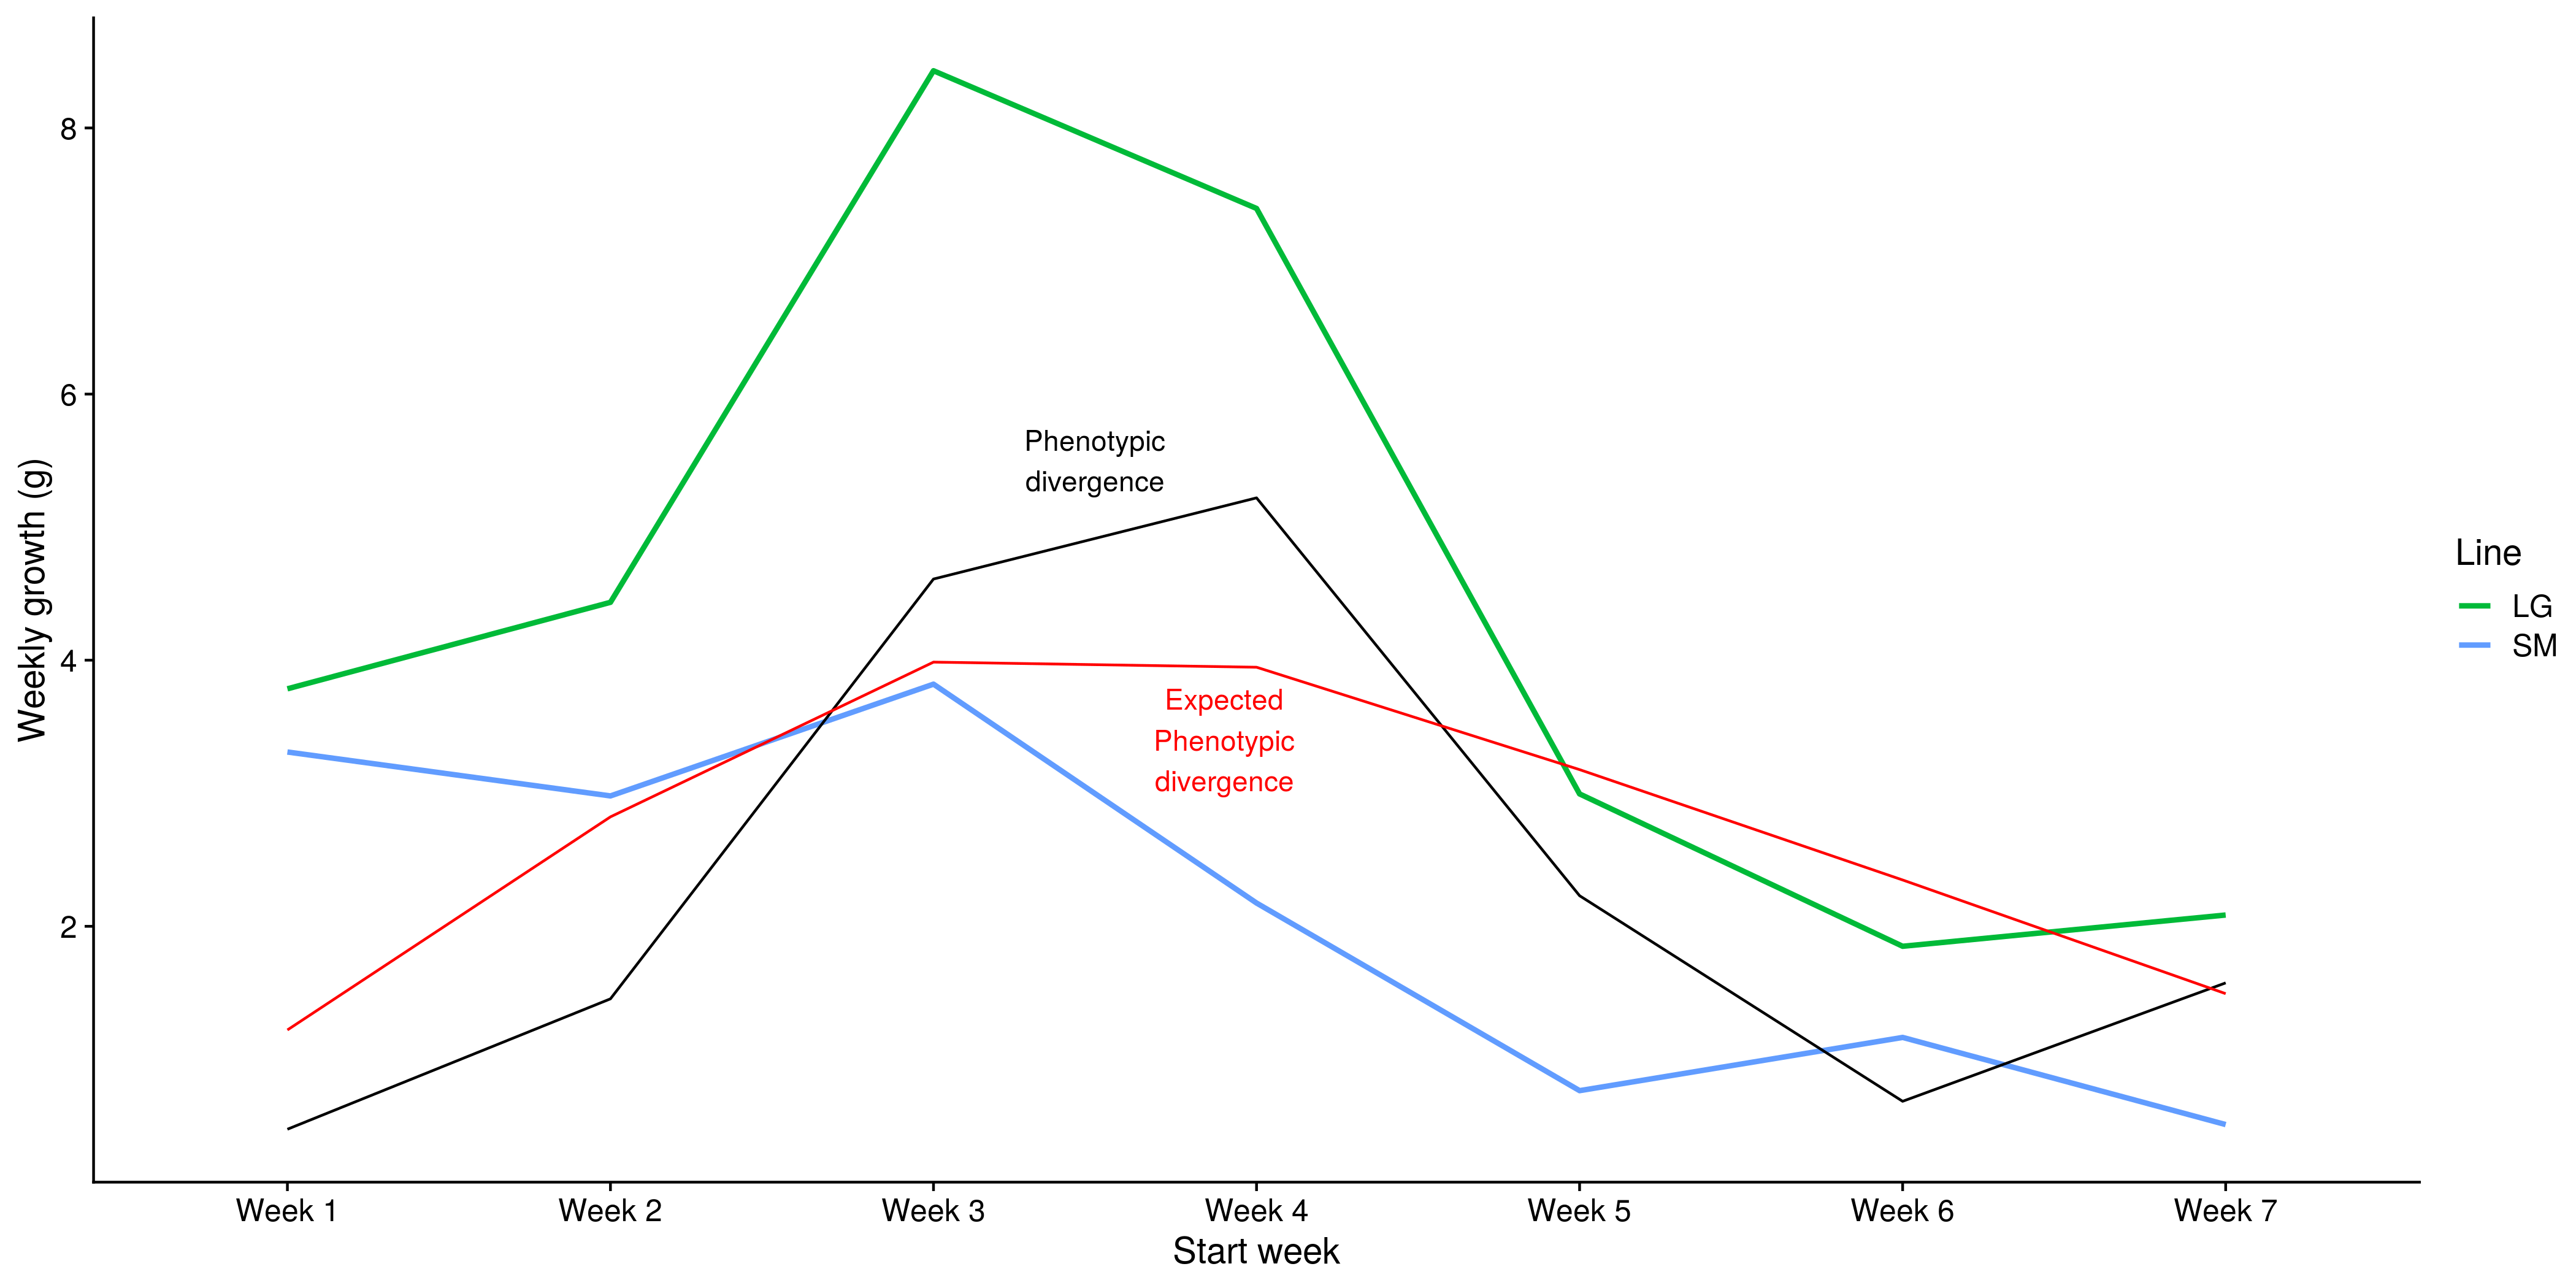
\includegraphics[width=\linewidth]{chapter_JoH-Melo_etal/media/growth_LG_SM_DZ2.png}
`	\caption[Phenotypic divergence in growth]{Observed and expected phenotypic divergence in the
parental lines. Expected divergence is estimated using the
F\textsubscript{3} generation to estimate a selection gradient on growth
due to selection on week 9 weight, and the expected divergence is
estimated by multiplying this selection gradient by the growth full-sib
genetic matrix. The resulting expected divergence is scaled to have the same
magnitude as the observed divergence.}
\label{fig:joh:divergence}
\end{figure}

\begin{figure}
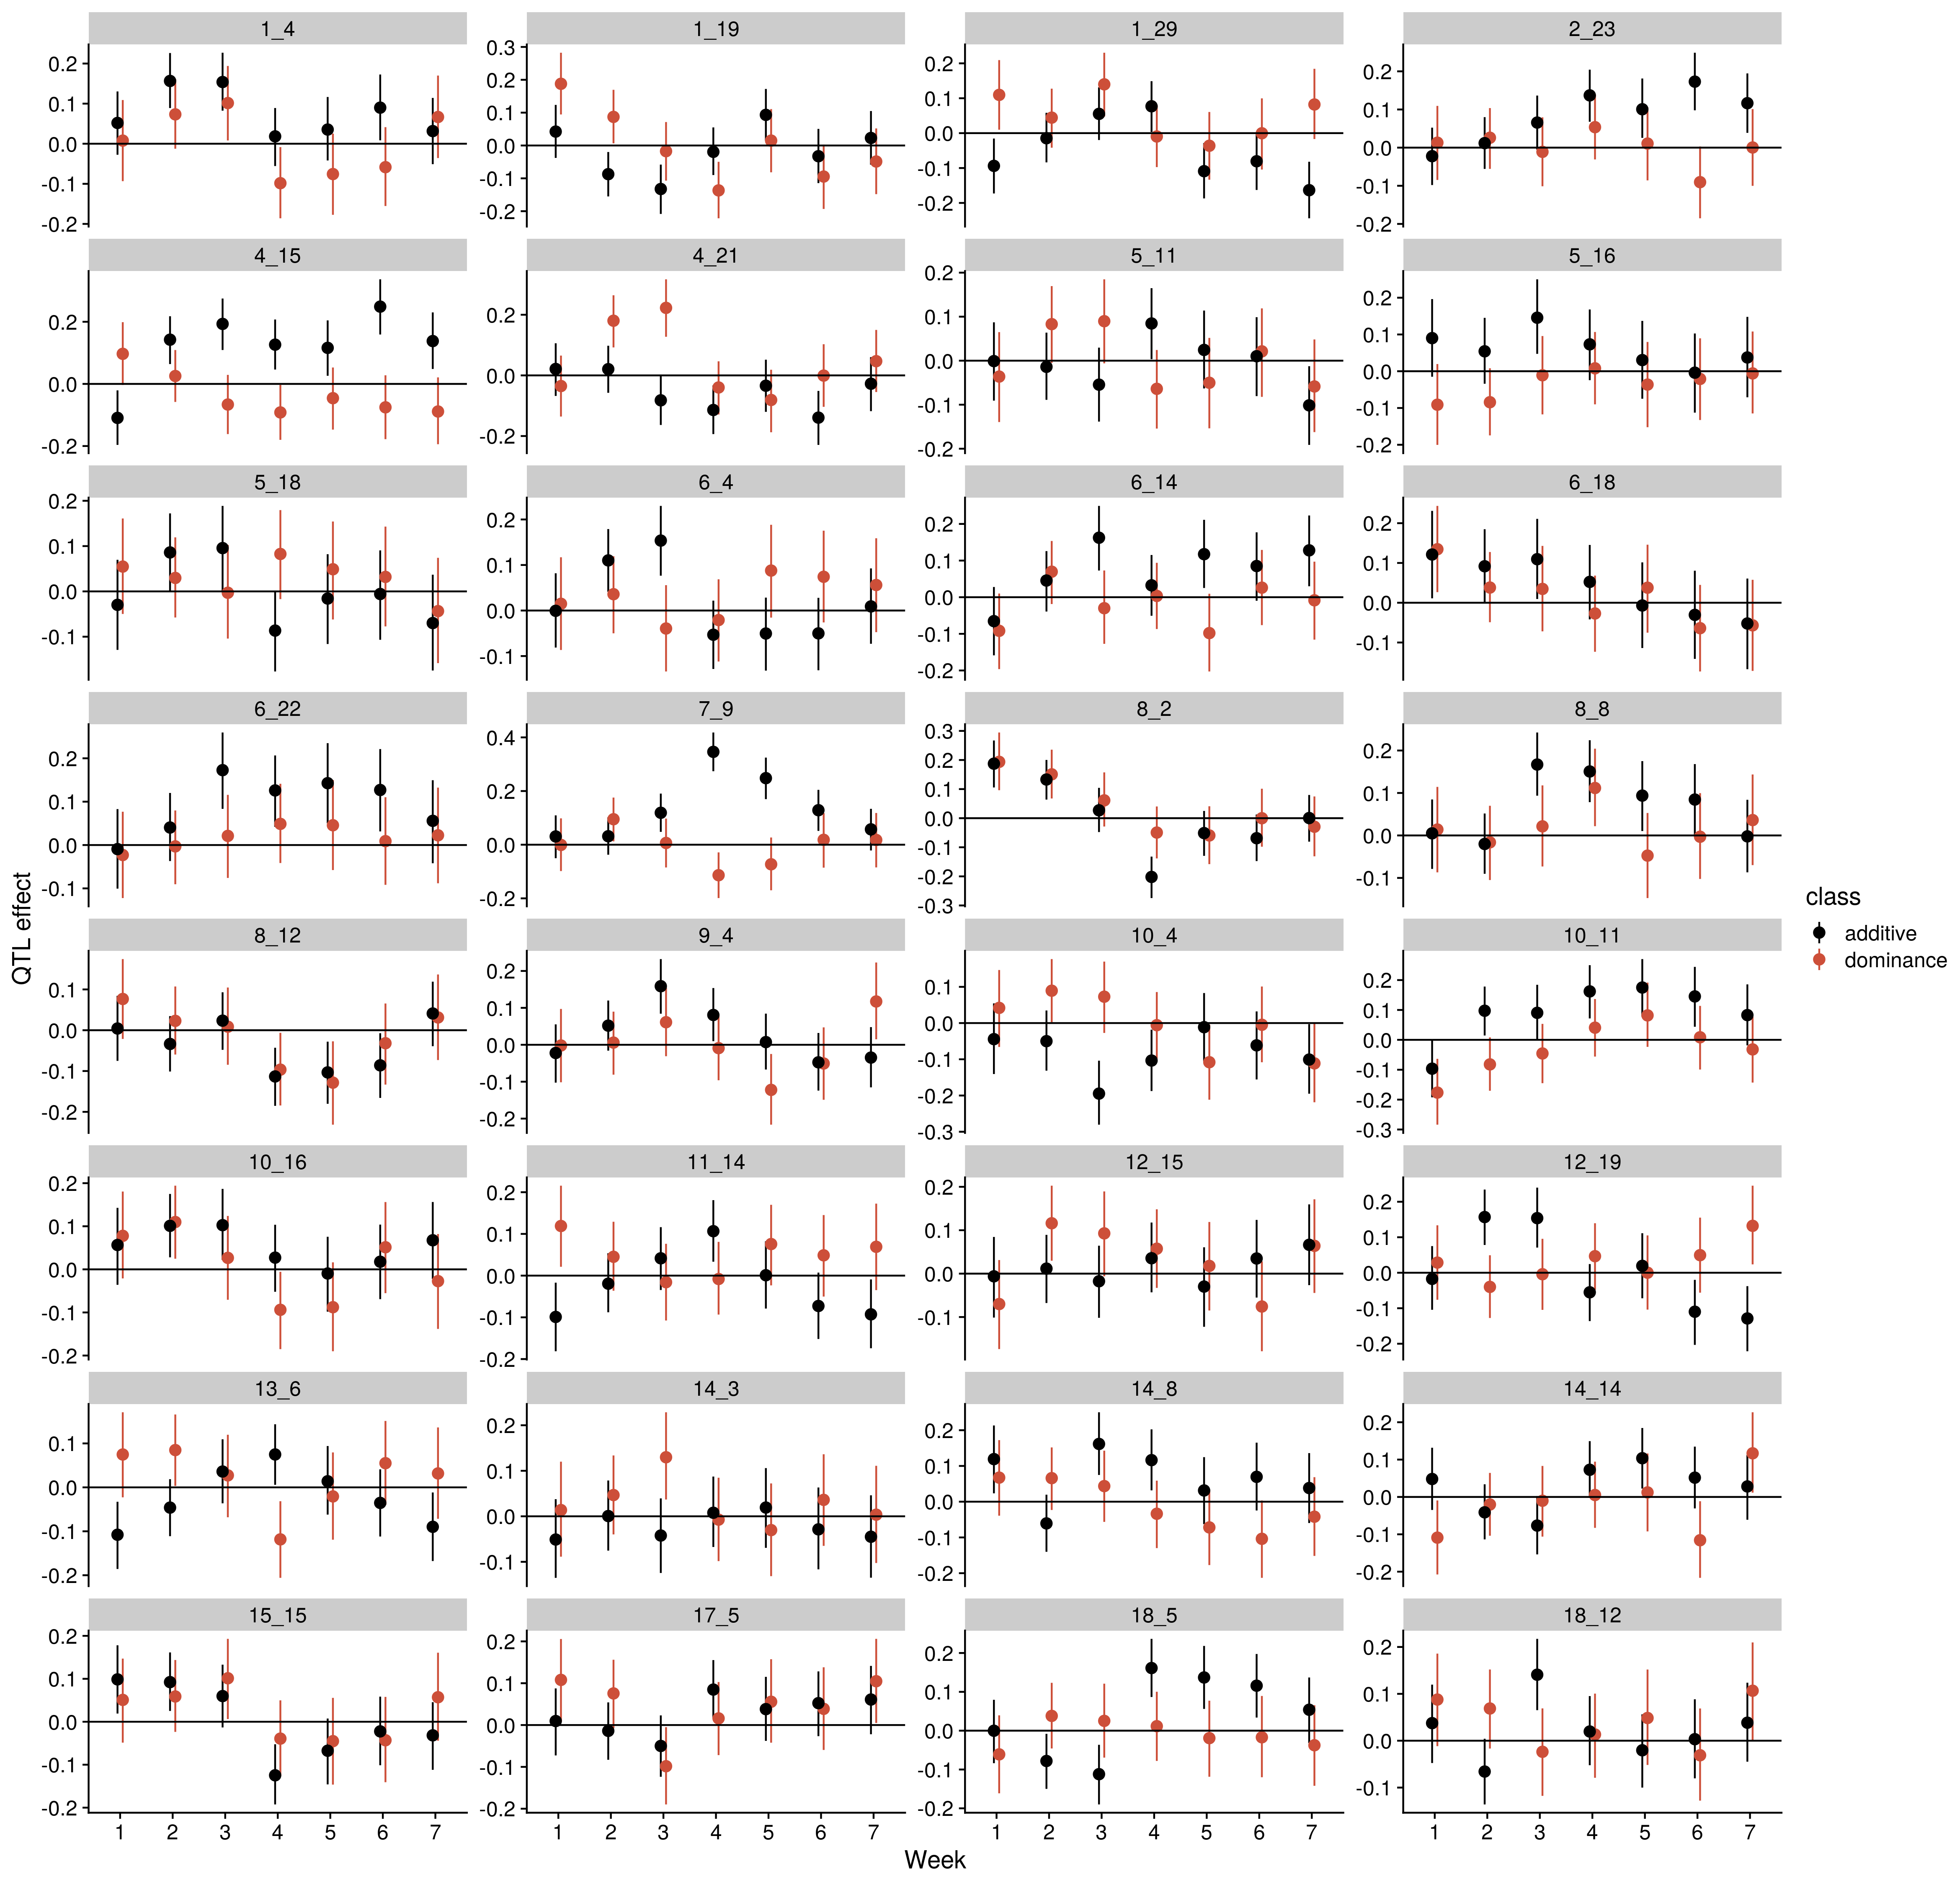
\includegraphics[width=\linewidth]{chapter_JoH-Melo_etal/media/growth_per_marker_additive_dominance_vectors_QTL.png}
\caption[Mapped pleiotropic effects]{Pleiotropic effects of all significant loci in the QTL
mapping model.}
\label{fig:joh:pleiovectors}
\end{figure}

\begin{figure}
	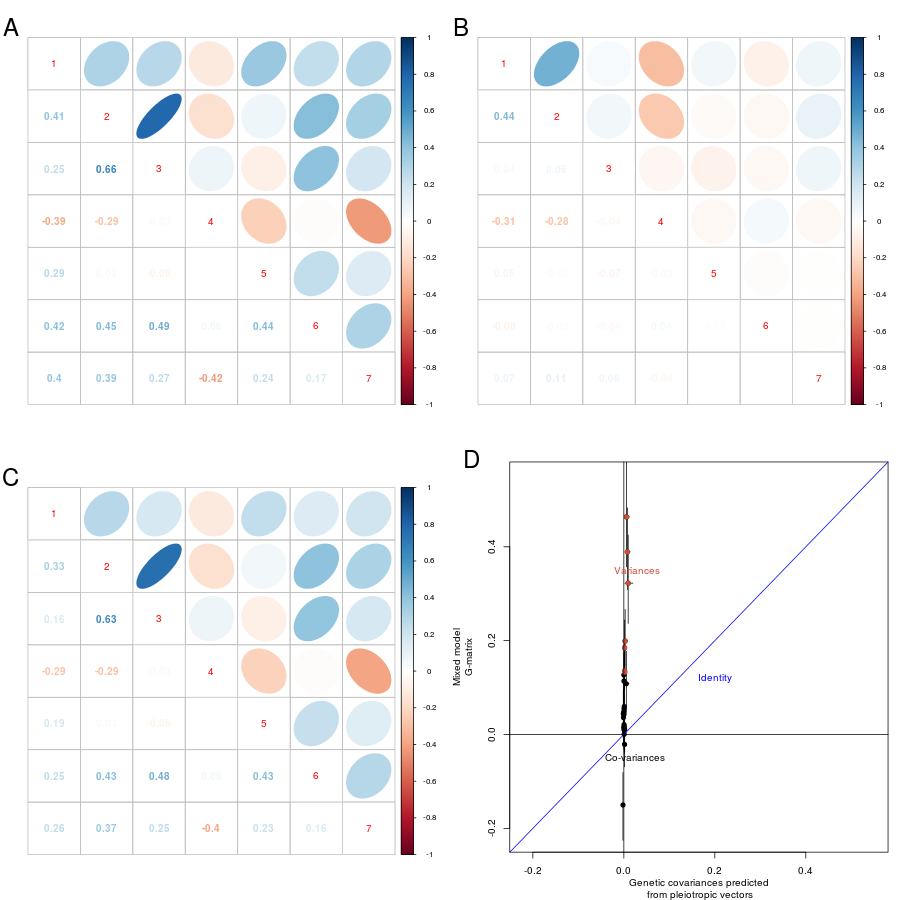
\includegraphics[width=\linewidth]{chapter_JoH-Melo_etal/media/growth_cov_prediction_composite_GP.png}
	\caption[Additive, dominance and genetic matrices]{Additive, dominance and genetic matrices.
	Estimated correlation matrices from genome prediction marker effects. (A)
additive, (B) dominance (C) Genetic, ½ additive + ¼ dominance . (D)
Regression of genetic variances and covariances estimated from full-sib
mixed model and estimated from markers. Error bars represent 95\%
posterior credibility intervals. All estimated variances are essentially
zero, and correlation matrices are different from the population
full-sib genetic matrix.}
\label{fig:joh:covGP}
\end{figure}

\end{refsection}
